\documentclass[f,bachelor,binding,twoside,palatino]{WeSTthesis}
% Please read the README.md file for additional information on the parameters and overall usage of WeSTthesis

\usepackage[english, ngerman]{babel}        % English and new German spelling
\usepackage[utf8]{inputenc}                 % correct input encoding
\usepackage[T1]{fontenc}                    % correct output encoding
\usepackage{graphicx}                       % enhanced support for graphics
\usepackage{tabularx}                       % more flexible tabular
\usepackage{amsfonts}                       % math fonts
\usepackage{amssymb}                        % math symbols
\usepackage{amsmath}                        % overall enhancements to math environment
\usepackage[babel,german=quotes]{csquotes}
\usepackage{url}
\usepackage{glossaries}
\usepackage{xcolor}
\usepackage{float}
\usepackage{longtable}

\usepackage{listings}
\lstdefinelanguage{HTML5}{
  language=HTML,
  morecomment=[s]{<!-}{-->},
  tag=[s],
  otherkeywords={lare-head, lare-body, lare-namespace}
}
\lstset{language=HTML5}

\makeglossaries

\usepackage{glossaries}

\newglossaryentry{ajax}
{
  name=AJAX,
  description={Asynchronous JavaScript and XML \footnote{\url{https://developer.mozilla.org/de/docs/AJAX}}}
}

\newglossaryentry{djangoLare}
{
  name=django-lare,
  description={The \lare{} backend for django}
}

\newglossaryentry{dynamicWebPage}
{
  name=dynamic web page,  
  description={A dynamic web page is a web page that is generated by a web application on a web server before it gets delivered.}
}

\newglossaryentry{hijax}
{
  name=HIJAX,
  description={Hijax}
}

\newglossaryentry{html}
{
  name=HTML,
  description={HTML stands for Hyper Text Markup Language and is the language that is used in the Web.}
}

\newglossaryentry{httpRequest}
{
  name=HTTP request,
  description={Hypertext Transfer Protocol requests build the foundation for data communication in the World Wide Web.}
}

\newglossaryentry{lareJS}
{
  name=lare.js,
  description={lare.js is the \lare{} frontend and the \ajax{} engine for \lare{}.}
}

\newglossaryentry{phpLare}
{
  name=PHP-lare,
  description={PHP-lare is the \lare{} backend for PHP.}
}

\newglossaryentry{lare}
{
  name=Lare,
  description={Lightweight asynchronous replacement engine is a technology for stateful \singlePageApplication{}s.
  It consists of a \lare{} frontend as ajax engine, and a \lare{} backend which is plugged into the web application.}
}

\newglossaryentry{singlePageApplication}
{
  name=single-page application,
  description={A single-page application is a web application or web site that retrieves one full \webPage{}.
  Beside this first page load, the web site is not loaded completely at any point in the process anymore.
  Often content changes are made asynchronous and dynamically by \ajax{} in response to user actions.}
}

\newglossaryentry{staticWebPage}
{
  name=static web page,
  description={A static web page is a web page that is delivered exactly as stored in the web server's file system.}
}

\newglossaryentry{twig}
{
  name=Twig,
  description={Twig}
}

\newglossaryentry{twigLare}
{
  name=Twig-lare,
  description={Twig-lare is the \lare{} backend for Twig and uses \phpLare{}.}
}

\newglossaryentry{url}
{
  name=URL,
  description={A Uniform Resource Locator identifies and defines the location of a resource, e.g. a \webPage{}.}
}

\newglossaryentry{w3c}
{
  name=W3C,
  description={The World Wide Web Consortium (W3C) is an international community where Member organizations, a full-time staff, and the public work together to develop Web standards. Led by Web inventor Tim Berners-Lee and CEO Jeffrey Jaffe, W3C's mission is to lead the Web to its full potential.\footnote{http://www.w3.org/Consortium/}}
}

\newglossaryentry{webApplication}
{
  name=web application,
  description={A web application is a application that generates \webPage{}s.}
}

\newglossaryentry{webPage}
{
  name=web page,
  description={A web page is a single document and part of a web site. 
  Every page should be accessible over the Internet and has it's own URL.
  A web browser can retrieve web pages by making \httpRequest{}s and it can render them afterwards.}
}

\newglossaryentry{webSite}
{
  name=web site,
  description={A web site is a collection of \webPage{}s that are linked to each other.}
}




% terminology definitions
\def \ajax {\gls{ajax}}
\def \clientSideMVC{client-side MVC}
\def \ClientSideMVC{Client-side MVC}
\def \djangoLare {\gls{djangoLare}}
\def \hijax {\gls{hijax}}
\def \html {\gls{html}}
\def \http {HTTP}
\def \httpRequest {\gls{httpRequest}}
\def \lareJS {\gls{lareJS}}
\def \LareJS {\Gls{lareJS}}
\def \lare {\gls{lare}}
\def \phpLare{\gls{phpLare}}
\def \singlePageApplication {\gls{singlePageApplication}}
\def \SinglePageApplication {\Gls{singlePageApplication}}
\def \twig {\gls{twig}}
\def \twigLare {\gls{twigLare}}
\def \webApplication {\gls{webApplication}}
\def \webPage {\gls{webPage}}
\def \WebPage {\Gls{webPage}}
\def \webSite {\gls{webSite}}


\author{Jonas Braun}

\title{\lare{} - A new technology for stateful \singlePageApplication{}s}

\degreecourse{Informatik}

\firstreviewer{Prof. Dr. Steffen Staab}
\firstreviewerinfo{Institute for Web Science and Technologies}

\secondreviewer{Ren\'e Pickhardt}
\secondreviewerinfo{Institute for Web Science and Technologies}


\begin{document}

% optional: change document language from ngerman to english
\selectlanguage{english}

\maketitle
\pagenumbering{roman}


\selectlanguage{english}
\begin{abstract}
The aim of this thesis is to improve and benchmark \lare{} - A new technology for stateful \singlePageApplication{}s.
\lare{} is a front- and backend technology, developed on top of PJAX and the successor of PJAXR to easily improve \webSite{}s with the use of \ajax{} but without the disadvantages of it regarding browser functionality, SEO and user experience.

The thesis first presents \lare{} and describes how a realisation of it ideally should be structured. 
In a second stage a PHP backend, called \phpLare{} and the matching Twig extension \twigLare{} are introduced using those concepts. 
Additionally the existing JavaScript frontend \lareJS{} and the django backend \djangoLare{} are refactored to match those guidelines, too.
Finally \lare{} gets evaluated in form of benchmarks using \curl{} for plain \httpRequest{}s and \selenium{} for retrieving \webPage{}s including all resources. 
For this purpose a sample web application is implemented using PHP, Twig and the matching \lare{} plugins.

The results of this evaluation show that \lare{} satisfies it's expectations regarding browser functionality and improves the load times of \singlePageApplication{}s.
\end{abstract}

\selectlanguage{ngerman}
\begin{abstract}
Ziel dieser Thesis ist es \lare{} - eine neue Technologie f\"ur stateful \singlePageApplication{}s zu verbessern und auf Geschwindigkeit zu testen.
\lare{} ist eine auf PJAX basierende front- und backend Technologie die als Nachfolger von PJAXR entwickelt wurde um einfach \webSite{}s mit \ajax{} Unterst\"utzung zu entwickeln, aber ohne die Nachteile im Bereich Browser Funktionalit\"at, SEO und User Experience.

Die Thesis pr\"asentiert anfangs \lare{} und beschreibt wie eine Realisierung idealer Weise strukturiert sein sollte.
In einem zweiten Schritt werden ein PHP backend, genannt \phpLare{} und eine passende Twig extension \twigLare{} eingef\"uhrt, die diese Konzepte nutzen.
Zus\"atzlich werden das existierende JavaScript frontend \lareJS{} und das django backend \djangoLare{} in Hinsicht dieser Richtlinien \"uberarbeitet.
Abschlie\ss{}end wird \lare{} in Form von Benchmarks mit Hilfe von \curl{} f\"ur reine \httpRequest{}s und \selenium{} zum empfangen kompletter \webPage{}s, inklusive aller Ressourcen, evaluiert.
F\"ur diesen Zweck wurde eine Beispiel \webApplication{} basierend auf PHP, Twig und den passenden \lare{} Plugins implementiert.

Die Ergebnisse dieser Evaluation zeigen, dass \lare{} die Erwartungen bez\"uglich Browser Funktionalit\"at erf\"ullt und die Ladezeiten von \singlePageApplication{}s verringert.
\end{abstract}
\selectlanguage{english}

\tableofcontents

\varclearpage

% list of figures
% \listoffigures
% \varclearpage

\pagenumbering{arabic}

\newcommand\todo[1]{\textcolor{red}{#1}}

\newpage{}

\section{Introduction}
At the beginning of the World Wide Web \webPage{}s were self-contained. 
And without a lot of effort they still are. 

The content of a \webPage{} which is initially loaded is not changed until a new resource is requested by the user.
One big change brought the invention of Asynchronous JavaScript and XML (\ajax{}). It introduced the possibility to change content without the need of requesting a full new \webPage{} on a different Uniform Resource Locator (URL).
The approach only loading one full \webPage{} initially and then changing its content interactively is called \singlePageApplication{}.
As presented in \cite{bib:jonsson09} page 26f. \singlePageApplication{}s are more user-friendly than the common designs, e.g. due to lower load times and the elimination of interruption time experienced on common \webApplication{}s.
\ajax{} is nowadays, other than mentioned in \cite{bib:jonsson09} page 27, available in nearly every browser.
As stated in \cite{bib:gov_uk13} in 2013 only 1.1\% of the internet users visiting the \webSite{} of the UK government did not get their JavaScript enhancements.

As mentioned in \cite{bib:jonsson09} page 27 a disadvantage of \ajax{} is that users are not able to save their websites as a bookmark, because while surfing on this page, the URL never changes.
Another implication stated there is that the functionality of back and forward buttons in browsers is often not given.
Additionally \ajax{} driven \webApplication{}s may require multiple small server calls which might produce performance implications.

\singlePageApplication{}s have another problem in the current time. 
As mentioned in \ref{matter:09} p. 13 \ajax{} websites are difficult to examine for search engines and other crawlers, due to several challenges.

As Google is the most used search engine in the World Wide Web they have a design pattern\footnote{https://developers.google.com/webmasters/ajax-crawling/docs/getting-started (Accessed: Juli 22, 2015)} for implementing a crawlable \ajax{} web application.
In this guideline it is recommended to have snapshots available under non-user-friendly \gls{url}s, called Hash-Bang URLs.
This means additional maintenance effort for \webSite{}s, especially when they are very dynamic.

In this thesis we will improve and evaluate the performance of a new technology called \lare{}.
Together with Stephan Gro{\ss} the author developed PJAXR the predecessor of \lare{} for using \ajax{} with it's advantages but trying to avoid the disadvantages explained before.

The result of this cooperation was a frontend-side implementation called \emph{jquery-pjaxr}.
As PJAXR also needs a backend to be implemented, I developed the first PJAXR backend called \emph{django-pjaxr}.

The libraries \lareJS{} and \djangoLare{} are introduced in this thesis as the successors of \emph{jquery-pjaxr} and \emph{django-pjaxr}.
Additionally in this thesis the author will introduce a new \lare{} backend for PHP, \emph{\phpLare{}} and \emph{\twigLare{}} an extension for the \twig{}\footnote{http://twig.sensiolabs.org/} template-engine.

Later \lare{} will be evaluated to see whether the expectations regarding browser functionality are satisfied.
Furthermore the performance will be tested through benchmarks using Curl and Selenium in combination with webdrivers, to see whether \lare{} is faster than normal web requests.


\newpage{}

\section{Fundamentals}

To understand how \lare{} works a few technologies are required to know about.
\html{}, the markup language which is used to create \webPage{}s, is the first technology which is mentioned in this chapter.
Afterwards \httpRequest{}s are presented as the fundamental transfer protocol of the World Wide Web.
Dynamic content and synchronicity are the topics explained next, the problem addressed by \ajax{} and \singlePageApplication{}s, which are presented subsequently.
The History API, released in October 2014, is required by \lare{} and presented at the end of this chapter.

\subsection{\html{}\label{html}}
Hypertext Markup Language (\html{}) is the language which is used to create webpages.
It's specification is defined by the \gls{w3c}\footnote{http://www.w3.org/TR/html5/ (Accessed: June 24, 2015)}.
It allows to structure a web document semantically, but not to style it.
Similar to XML it consists of hierarchically structured tags.
Each tag may have attributes.
Allowed attributes are defined per tag, e.g. an anchor tag (<a>) may have an href attribute, which is not allowed on a div tag (<div>).
This href attribute defines where the anchor should lead to, when clicked on.
\\
Another type of attributes are the data attributes.
It is a attribute whose name starts with the string \enquote{data-} followed by at least one other character.
Those attributes are intended to store custom information, for which there are no more appropriate attributes or elements.
\\
There is a special attribute called \enquote{id} which defines the unique identifier of a tag.
Each value of it may not occur more than once on a \webPage{}.

\subsection{\httpRequest{}s\label{httpRequest}}
The World Wide Web has one main protocol to let \webBrowser{}s and \webServer{}s communicate, the Hypertext Transfer Protocol (\http{}), which is built on top of the Transmission Control Protocol (TCP).
TCP and so \httpRequest{}s always start with a handshake to establish a connection before data is transferred.
After this handshake, the client sends the request data to the \webServer{}.
This recognizes and interprets the request and if the requested resource is available, sends the according data back, otherwise it sends an error.
\WebApplication{}s typically render data out of a database into a \html{} template and sends it back as the response.
The browser receives this \webPage{} interprets and renders it.
Subsquently it sends \httpRequest{}s to receive the images, Cascading Style Sheets (CSS) and scripts linked in this page.
\begin{figure}[H]
\centering
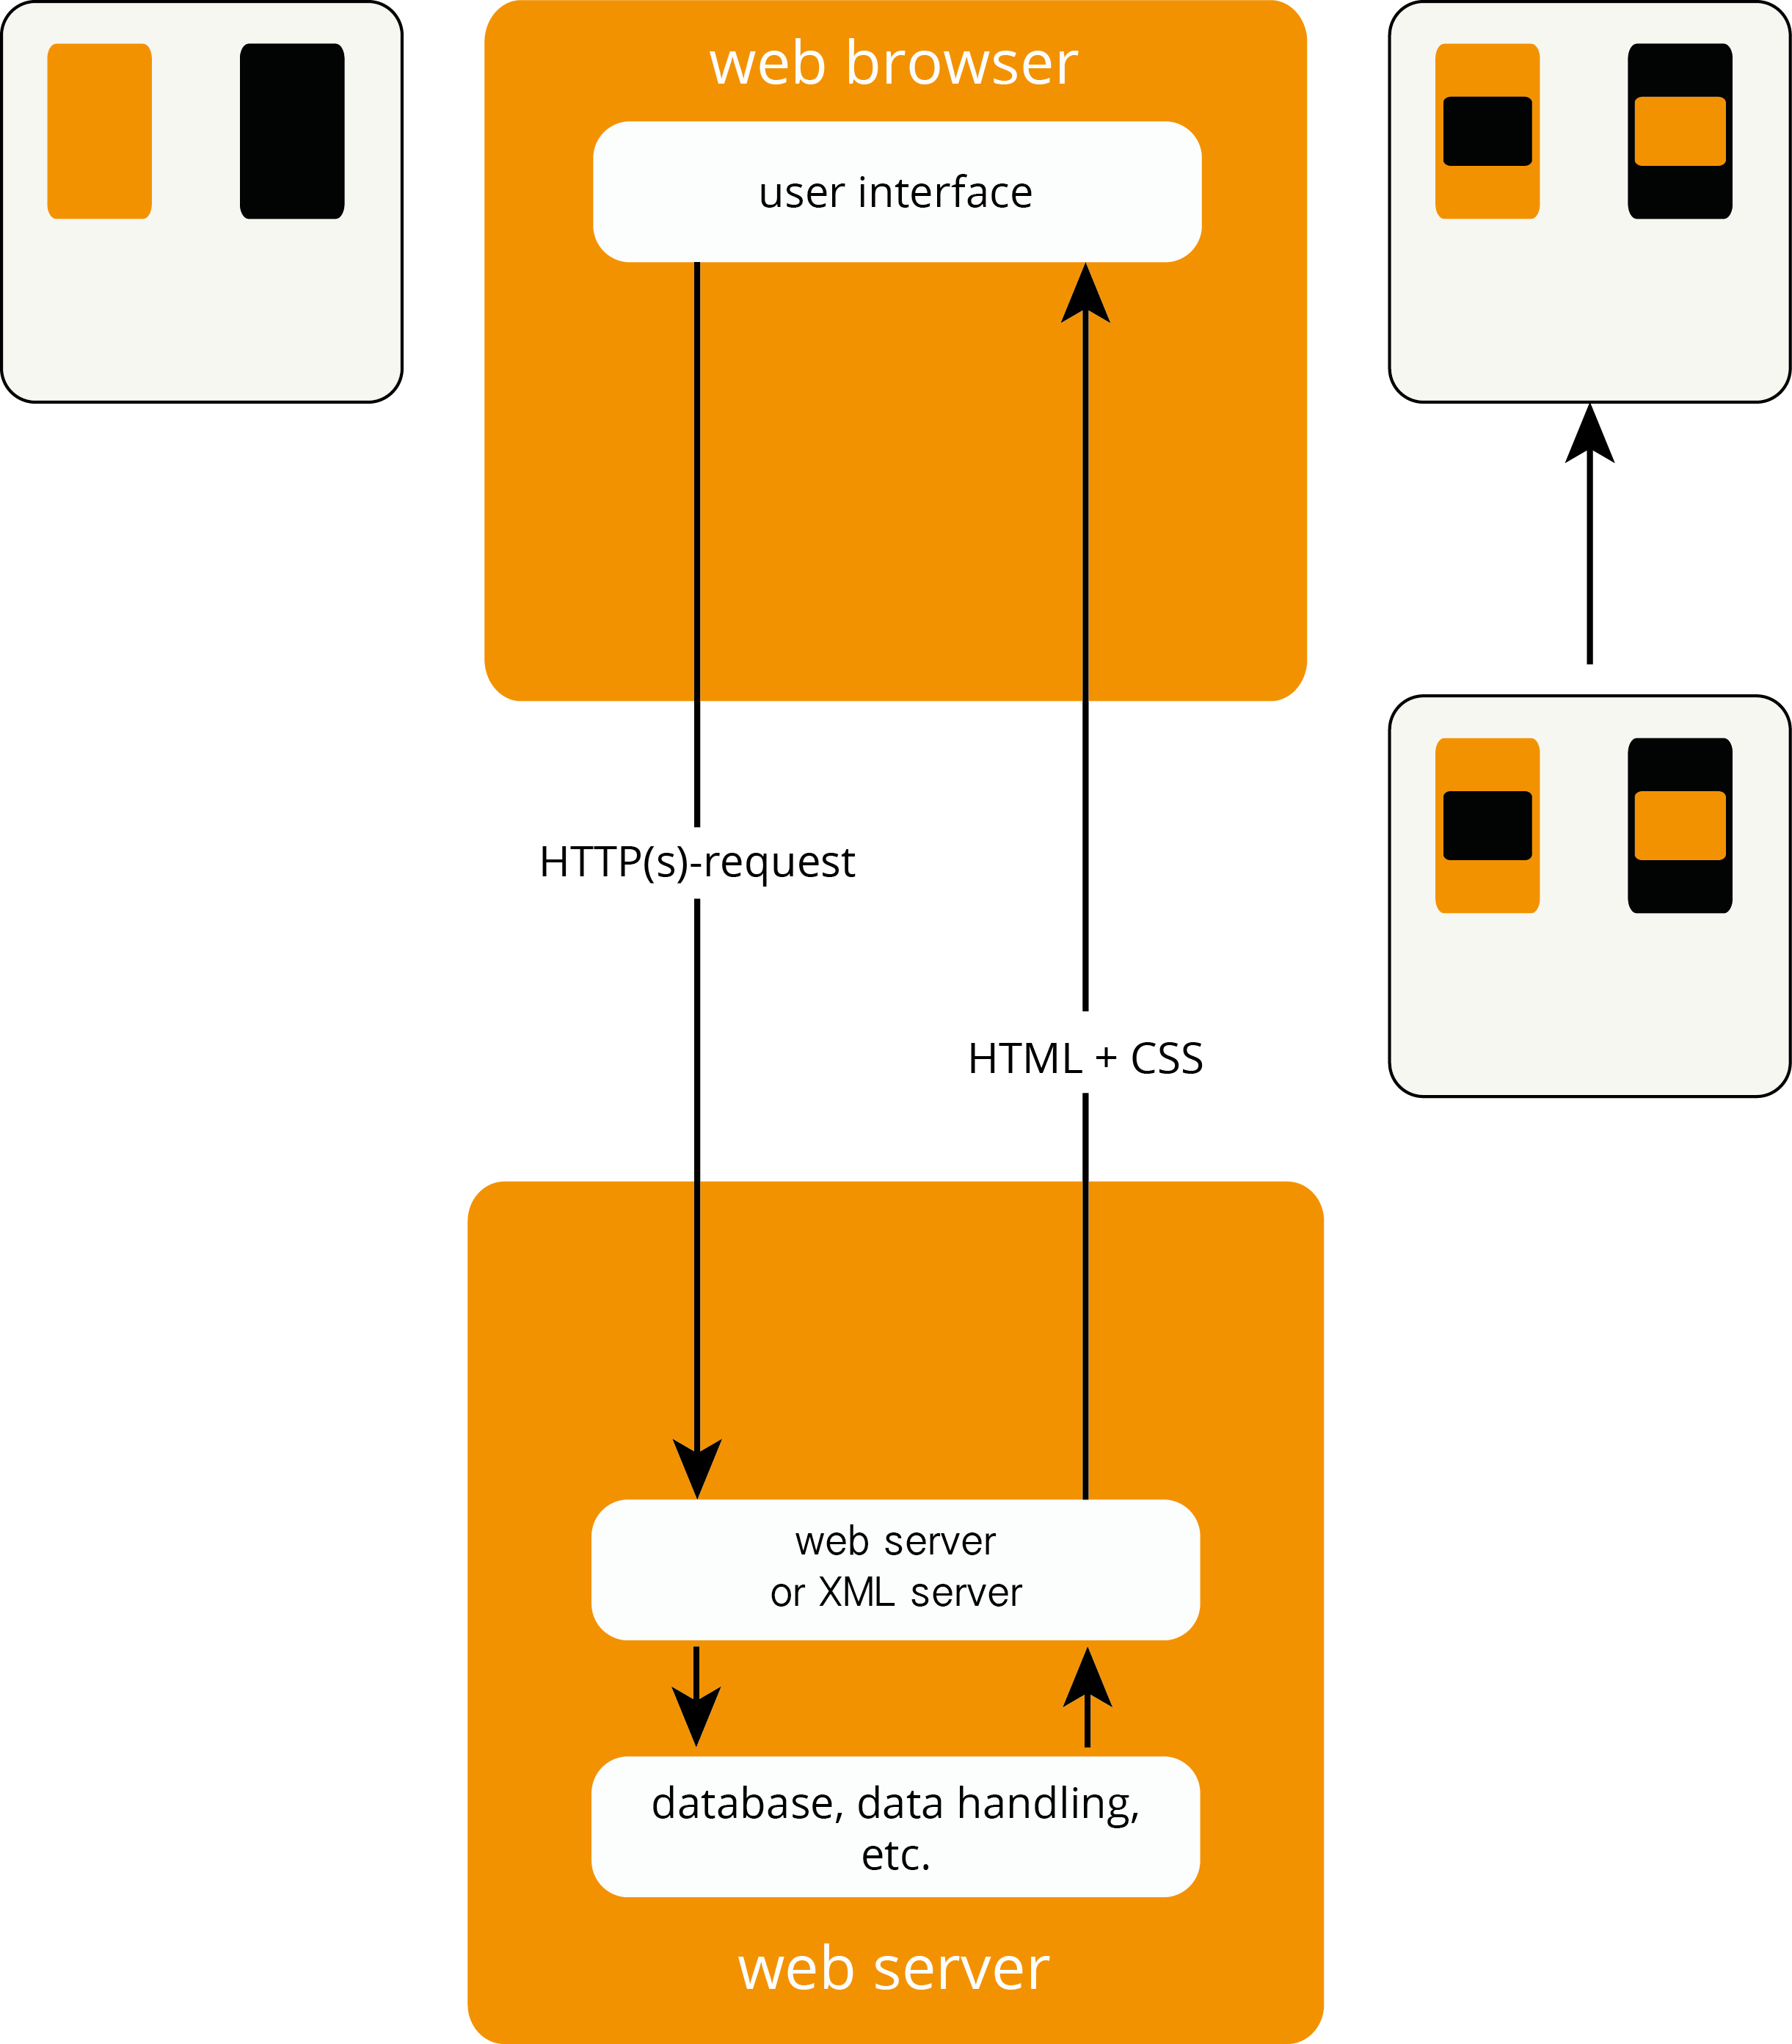
\includegraphics[height=13cm]{images/http.png}
\caption[http_components]{Component and communication diagram of \http{}}
\label{fig:http_components}
\end{figure}

\noindent{}Figure \ref{fig:http_components} displays this communication of a \webBrowser{} and a \webServer{}.
On the top left you see a abstract representation of a \webPage{}.
On the right side in the middle you can see the response, in this case a complete new \webPage{}, which then replaces the previous from the top left completely.


\subsection{Dynamic content and synchronicity\label{synchronicity}}
Dynamic content in \webSite{}s is content which is changed within an already fully loaded \webPage{}, without loading another full page including all resources. 
The normal \httpRequest{}, which is described in \ref{httpRequest}, does not support dynamic changes of content. 
To retrieve new information the client has to request another full \webPage{}, including all resources and data which is necessary, which makes this model \enquote{synchronous}.
An \enquote{asynchronous} model is able to change content dynamically without having to load a whole page. 
\ajax{}, as shown in \ref{ajax}, is the most used technique for asynchronous \webSite{}s.

\subsection{\ajax{}\label{ajax}}
Asynchronous JavaScript and XML is a technology to implement dynamic \webPage{}s.
JavaScript is used to make requests to a \webServer{} without loading a full new page.
The response then is interpreted by an \ajax{}-engine.
\begin{figure}[H]
\centering
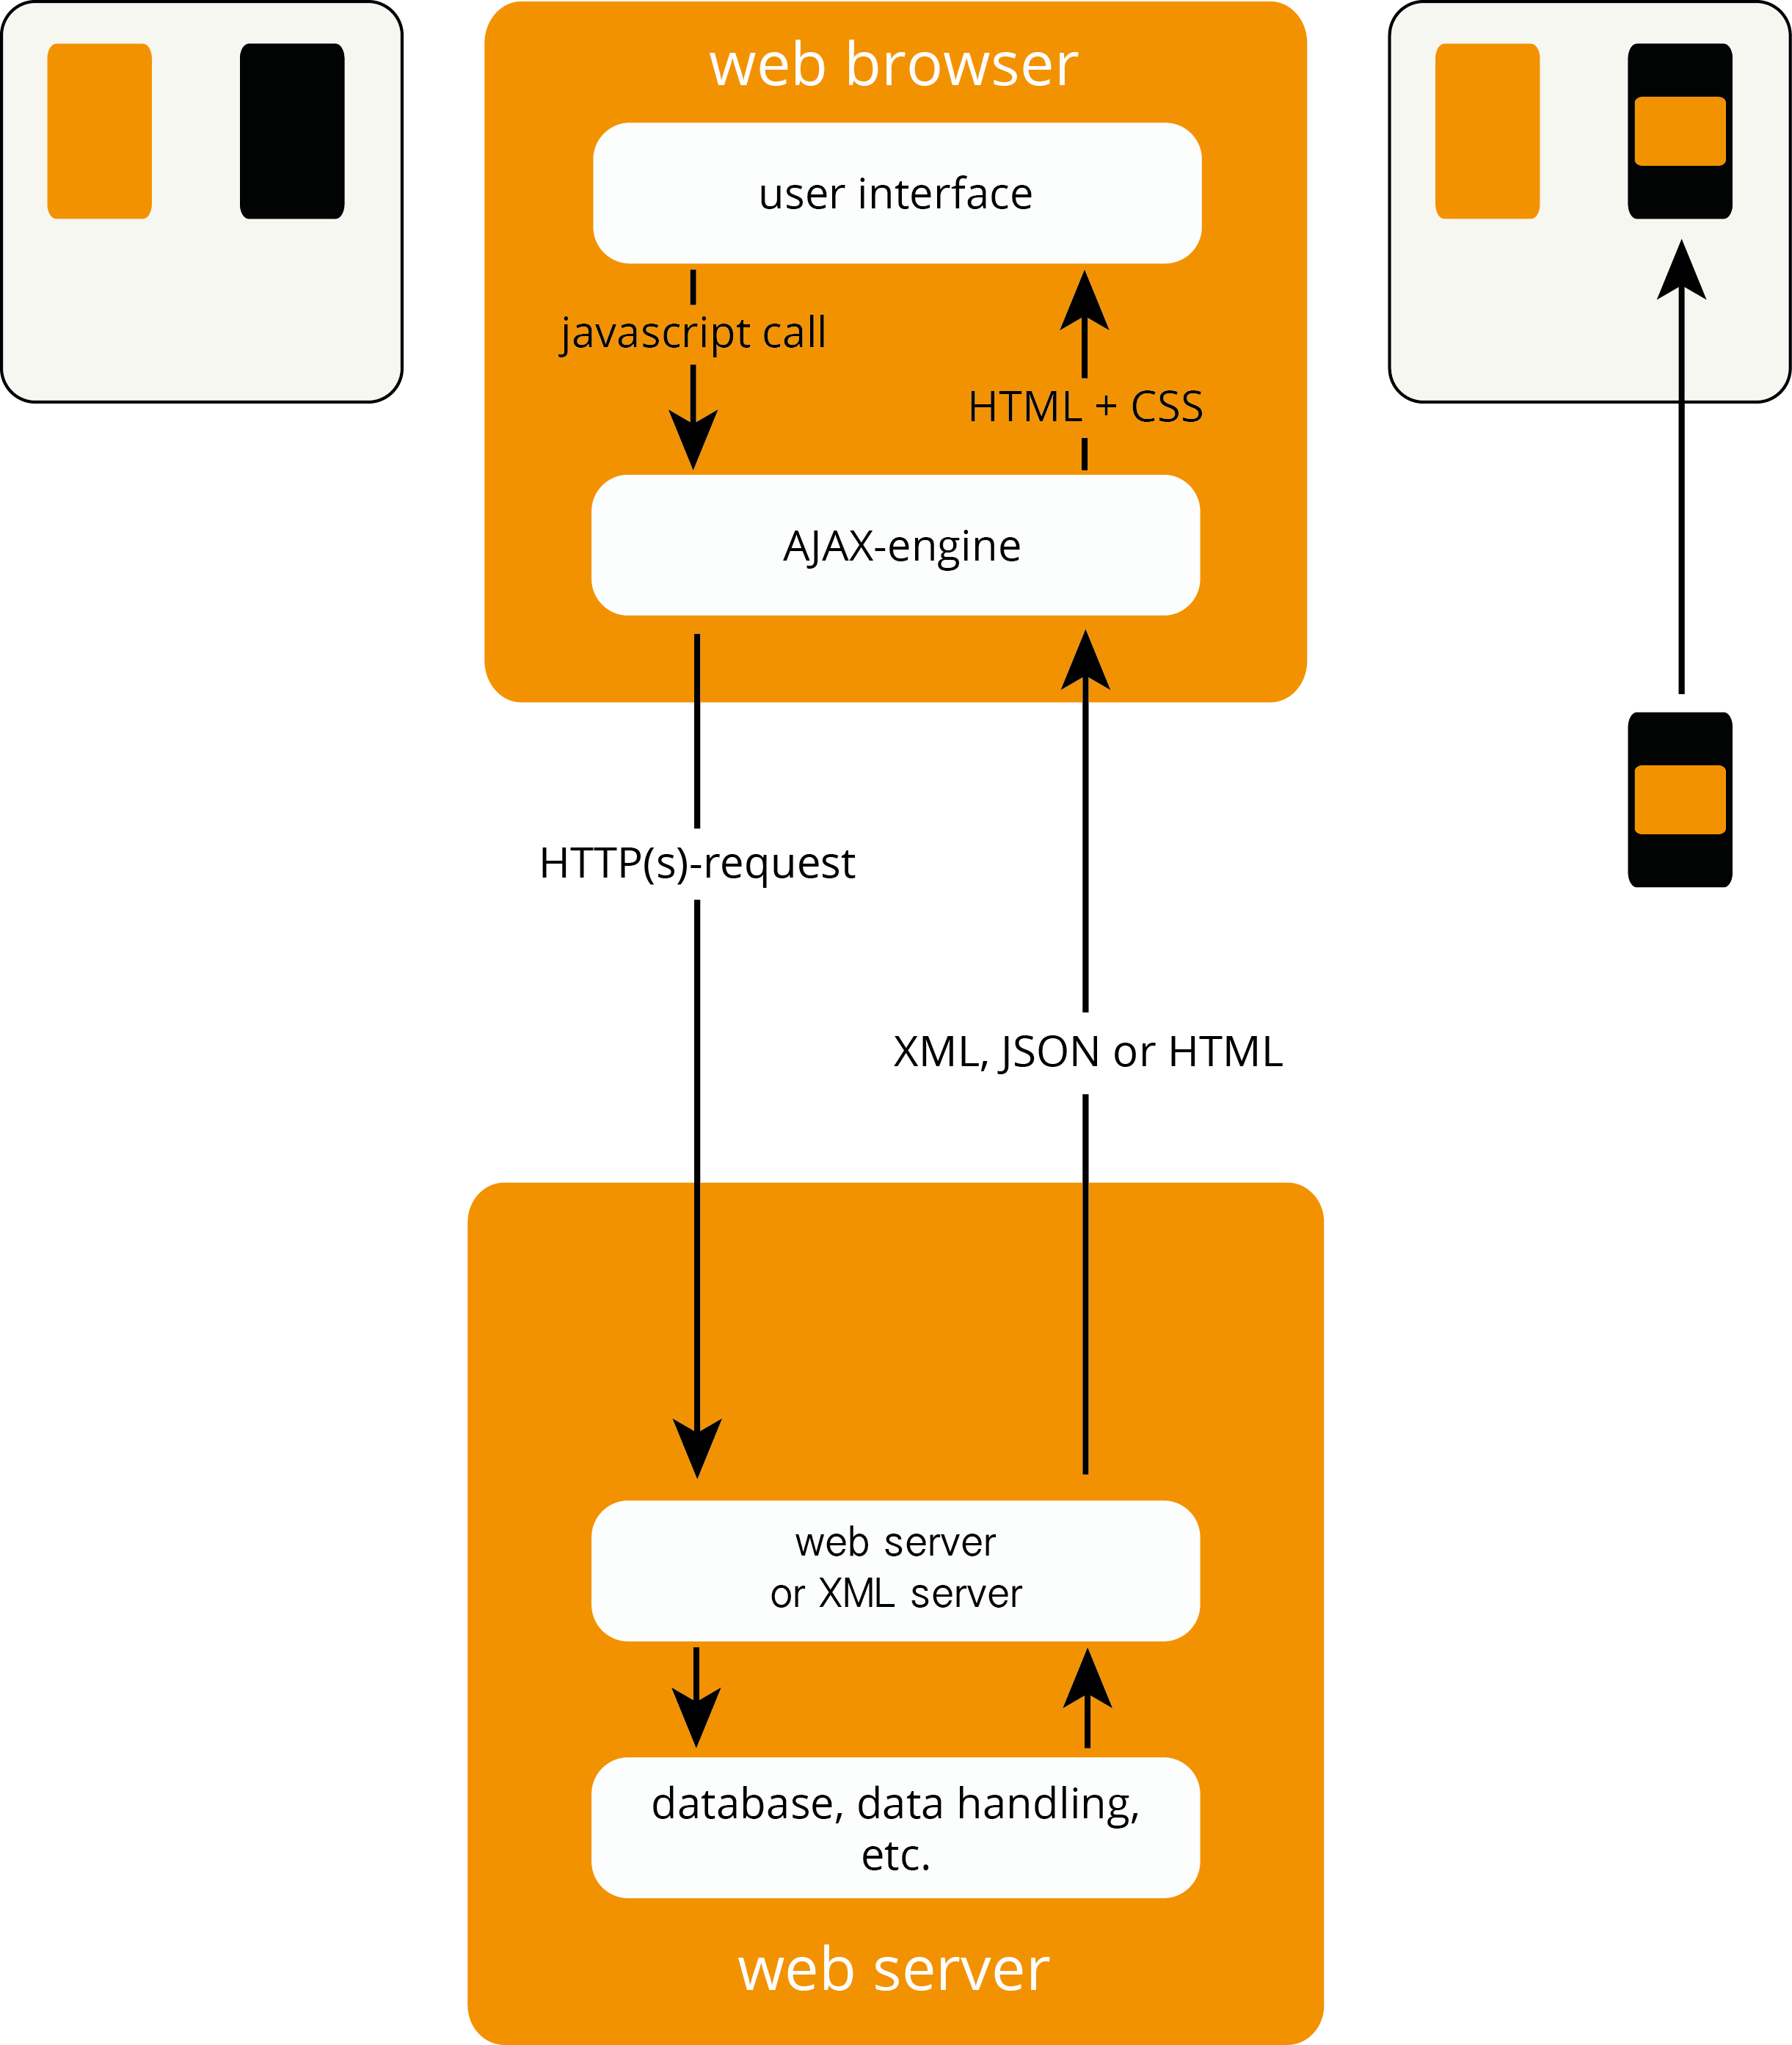
\includegraphics[height=13cm]{images/ajax.png}
\caption[ajax_components]{Component and communication diagram of \ajax{}}
\label{fig:ajax_components}
\end{figure}

\noindent{}As shown in fig. \ref{fig:http_components} a normal \http{} request by a browser forces the requests always to be synchronous, which means that the client has to wait for a fully loaded page on every request.
Through the \enquote{Asynchronous JavaScript and XML}, short \ajax{}, this can be improved.
The data flow in AJAX is very similar to the normal browser behaviour, but is using a new component: the \enquote{\ajax{}-engine}.
The first request to a \webServer{} using \ajax{} is the complete same as one without \ajax{} with the exception, that one of the requested sources is a JavaScript, which instantiates a \ajax{}-engine.
The following requests are handled by this \ajax{}-engine, allowing to asynchronously request content from the \webServer{}.
\ajax{} can request only small parts of a website, most of the time in XML or JSON format, interprets it and then only adds, replaces or appends old content with the newly received.
Figure \ref{fig:ajax_components} shows that only one part of a \webPage{} is responded and replaced, instead of the whole page in fig. \ref{fig:http_components}.

\subsection{\SinglePageApplication{}s\label{singlePageApplication}}
A \singlePageApplication{} (SPA) is a \webApplication{} or \webSite{} that only needs one full \webPage{} load.
Beside this there is no \webPage{} loaded completely at any point in the process anymore.
Often content changes are made asynchronous and dynamically by \ajax{} in response to user actions.
A disadvantage of a lot of \singlePageApplication{}s is the lack of browser history support.
When changing the content the browser does not interpret it as a new page, but only changed content.
This leads into a missing functionality of forward- and back-buttons in browsers.
\\
Additionally a problem of SPAs is, that it has a huge impact on SEO.
The \webPage{} is often rendered inside the browser, and not structured into different URLs.
Those facts make it hard for a search-engine to discover it.

\subsection{History API}
The History API is part of HTML5 specification by \gls{w3c}.
It describes the API for an History object which is part of the session history.
This session history enables functionality like the back and forward buttons on browsers.
Defined as a list of session history entries, it represents the browsing history.
A session history entry may be a URL or a state object and may have additional information.
\\
It is possible to influence this list via the window.history.pushState(data, title[, url]) method, which allows to add a new state into this list.
This also effects the browser's navigation bar, which gains the possibility for users to share or bookmark a \webPage{}.
\\

\newpage{}

\section{State of the art\label{chap:state_of_the_art}}
\ajax{} is a widely used technique in the internet to build web applications because of the user experience improvements it features.
In \cite{roodt2006effect} is mentioned that \ajax{} applications have a better usability than non-\ajax{} \webSite{}s.
The same conclusion is made in \cite{kluge2007effects}, despite the lack of browser navigation support.
Besides the navigation problem, another disadvantage is, as presented in \cite{mesbah2009analysis}, crawling \ajax{} applications is not trivial.
One solution to this task is finding clickables and navigating to every page found.
Nevertheless \cite{mesbah2009analysis} also states that this only generates a snapshot of the full application.
Even search engines are avoiding to crawl \webSite{}s because of it's difficulty\cite{duda2009ajax}.
Currently the task of building a crawlable \singlePageApplication{} using \ajax{} is often avoided. Instead crawling algorithms are improved and in focus of research. One example for this is  like \emph{ATUSO} \cite{mesbah2012invariant}.

\subsection{Client-side rendering\label{sec:state_client_side_rendering}}
When building an asynchronous web application it is possible to render the pages in the client or in the server.
A lot of \ajax{} applications use a JSON API which already predefines the outcome of this decision:
\\
JSON is sent by the server, interpreted and rendered by the \ajax{}-engine in the client.
An advantage of this practice is the strong separation of the logic on the server and views on the client-side.
This \webApplication{} design also reduces the server load as the computation of rendering the data is made in the client.
The overhead of HTML markup for styles and the UI is not sent for every \webPage{} anymore which additionally reduces the traffic.
As plain string modifications are difficult to maintain especially on large applications, client-side templates become more and more widespread.
\\
As the web server does not render \webPage{}s, it is hard to create snapshots for search engines.
Headless browsers like Phantom.js\footnote{\url{http://phantomjs.org/} (Accessed: Juli 28, 2015)} can render such pages and serve them for crawlers.
\\
Figure \ref{fig:frontend_snapshots} shows the flow of a request by a crawler with the use of a headless browser and HashBang URLs, introcuded in \ref{hashbangurls}.
After the initial crawl request is made, the web server lets the server-side headless browser render a snapshot of the HTML and then response to the crawler with this snapshot.

\begin{figure}[H]
\centering
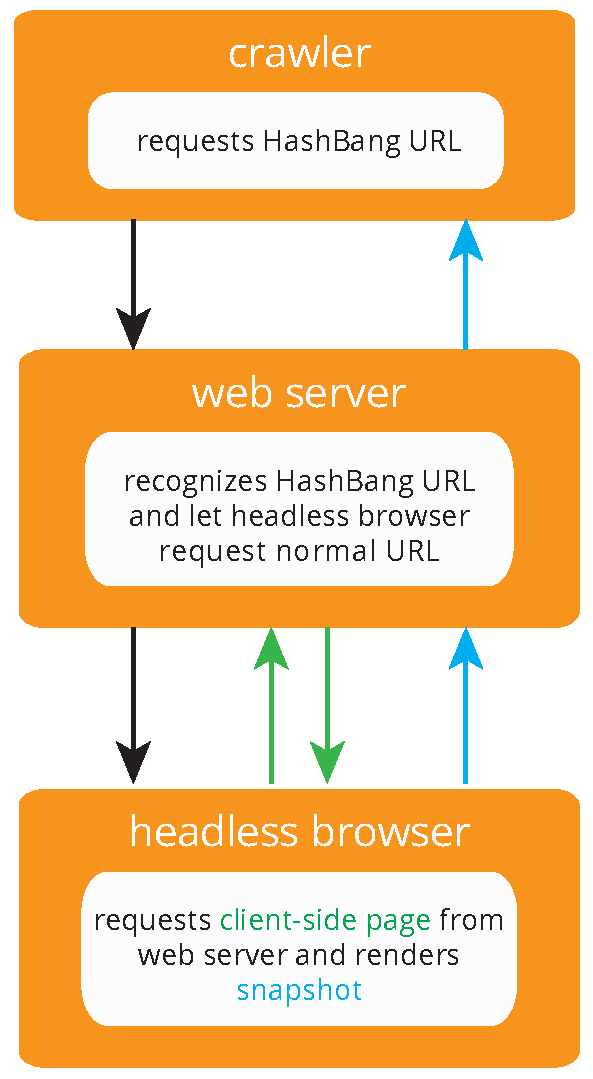
\includegraphics[height=10cm]{images/frontend_snapshots.pdf}
\caption[frontend_snapshots]{Rendering client-side rendered pages with headless browser}
\label{fig:frontend_snapshots}
\end{figure}

\subsubsection{Load time analysis}
With client-side rendering at least three requests are needed, before data is rendered:
\begin{enumerate}
    \item An HTML file containing a link to the \ajax{} engine and frontend templates.
    \item The \ajax{} engine itself.
    \item Data which should be rendered into the templates.
\end{enumerate}

\noindent{}It is not possible to run the three requests listed above in any other order or concurrently, because the \ajax{} engine is linked in the initial HTML file and the data gets requested by the \ajax{} engine.
\\
Sometimes the frontend templates must be requested additionally if they are not part of the HTML document or the AJAX engine.
Those template requests could be made concurrently to retriev the data, which is the reason that those further requests are ignored in the following analysis.
\\
To get a bit more into detail this means a series of requests and responses.
Mike Belshe states in \cite{belshe2010more} \enquote{More bandwidth doesn't matter (much)}.
Considering this and the fact he states that Round Trip Times influence the Web in a bigger way than bandwidth, we neglect data transfer in the following analysis.
\\
As HTTP is based on TCP it first has to make a handshake, which takes one RTT.
All of those three requests take at least one additional RTT, too.
This means it is necessary to wait at least four RTTs before the page starts to be rendered.
Taking the RTT of 70ms, used in \cite{spero1994analysis}, this means a waiting time of 280ms before rendering can start.
\\
An efficient \webApplication{} which uses client-side rendering requests one URL on which the response contains all needed data.
If more requests are needed an additional RTT per request has to be added to the example above.
\\
Despite the fact that the server could need additional time to render the page, common \httpRequest{}s need 2 RTTs less than this pattern.

\subsection{\ClientSideMVC{}\label{sec:state_client_side_mvc}}
In addition to only outsource the templating to the frontend, there are complete client-side MVC frameworks.
Those frameworks use the model view controller pattern, where the controller has a connection to the web server.
\\
Built on REST APIs\footnote{\url{http://www.peej.co.uk/articles/rest.html} (Accessed: Juli 28, 2015)} they move all logic into the client-side.
This approach is built primarily on the motivation to reduce the web server load and traffic.
\\
The initial request is divided into the three requests as shown in section \ref{sec:state_client_side_rendering}.
Further requests are not made to request URLs in the old fashioned way, but to retrieve objects through a REST API. 
Object manipulation, logical methods and everything normally implemented in a server backend should be in the frontend in those frameworks.
\\
Using this pattern, the same problems as with client-side templates will appear but on another level.
Instead of the web server, the client decides which information it needs and requests it from the server and renders those.
\\
Load and traffic of the server in this pattern is relatively low, because it will only create, update, delete or retrieve objects in the database. 
More logical functions on the server-side are not needed normally.
\\
Clients, especially mobile devices and slow computers, might struggle with the load of work instead.
\\
The most used client-side MVC framework is AngularJS\footnote{\url{https://angularjs.org/} (Accessed: Juli 28, 2015)}. In the evaluation in chapter \ref{chap:evaluation} it also represents this kind of \webApplication{}s.

\subsubsection{Load time analysis}
Similar to simple client-side templates mentioned in \ref{sec:state_client_side_rendering}, client-side MVCs need at least three requests to render the first page.
In most cases more than one model needs to be known by the client to render a page, which increases the amount of requests to render a page.
\\
To get into more detail, the client needs to wait for the first request to be completed, then the \ajax{} engine has to be loaded.
After the initialization of the \ajax{} engine, it requests the needed data.
\\
We are using 70ms as RTT as stated in \ref{sec:state_client_side_rendering} and get a result of 280ms for those three requests.
This result is the optimal result which can be achieved, but often it is much higher, because there is not one but multiple objects which have to be fetched independently.
It is not always possible to request all data concurrently, e.g. when a second object is linked in a first one.
In this case the first object has to be fetched and afterwards the second one if it's not known or linked before.

\subsection{Hash-Bang URLs\label{hashbangurls}}
In order to have a working SEO in SPAs it is recommended by Google to use hashbang URLs.
This pattern defines that in the URL the \emph{hash part} should start with \enquote{\#!} instead of only \enquote{\#}.
Finding this combination let crawlers know that the site provides an AJAX application and additionally full page snapshots created using techniques like shown in \ref{sec:state_client_side_rendering}.
When a crawler e.g. finds an URL like \url{http://example.com/\#!site=test1} it crawls \newline \url{http://example.com/?\_escaped\_fragment\_=site=test1} instead.
This is done, because everything after the \enquote{\#} will not be sent to the server, but is only recognized by the client.
To let the server know that a specific page should be requested this URL modification is needed.
At this \enquote{?\_escaped\_fragment\_=} URL a snapshot of the full page should be available.
This means, instead of only providing a few parts of the page required by \ajax{}, the whole HTML DOM should be delivered.
\\
On the other hand the \ajax{} engine can recognize everything behind the \enquote{\#} and requests the data needed for the page, lead to by the ongoing part.
\\
This technique was developed for URL changing by JavaScript without a full page reload.
Old browsers without the implementation of the History API are not able to change the URL without a full load of a page.
To gain navigation functionality on \singlePageApplication{}s the only way was to change the hash value in the URL, which does not call a page load, but updates the URL and pushes it to the navigation history.

\subsection{\hijax{}\label{hijax}}
Another way to implement \singlePageApplication{}s using \ajax{} is to use the development pattern of HIJAX.
When using PJAX and \lare{}, introduced in section \ref{sec:state_pjax} and chapter \ref{chap:lare}, the usage of this pattern is recommended.
\\
When developing a \webSite{} using this pattern, it should be planned with the use of \ajax{} but in the first step implemented serving just common \httpRequest{}s.
Changes of the HTML markup in favour of \ajax{} should be avoided at this step.
Every \webPage{} should be delivered fully and links should be linking to real \webPage{}s.
No JavaScript should be needed to link \webPage{}s within the site.
\\
After the \webSite{} is implemented completely the event listeners on the links can be \emph{hijacked} and processed by JavaScript.
A good way to do that is using classes in the linking tag which gain semantics in JavaScript.
This script then creates a new XMLHttpRequest which requests only the updated parts of the page and renders the response.
\\
When this pattern is used the \webSite{} degrades gracefully.
This means even when JavaScript is not available or blocked, the \webSite{} still works, a client can still discover the single pages and a crawler sees the whole content.

\subsection{PJAX\label{sec:state_pjax}}
PJAX, introduced 2011 by Chris Wanstrath, \enquote{is a jQuery plugin that uses AJAX and pushState to deliver a fast browsing experience with real permalinks, page titles, and a working back button.}\footnote{\url{https://github.com/defunkt/jquery-pjax\#introduction} (Accessed: Juli 28, 2015)}
Using it makes it possible to use the HIJAX pattern, introduced in \ref{hijax}.
\\
PJAX let the browser replace a container in a page by requesting a URL in a certain way like adding a \enquote{?pjax} query parameter.
When requesting a page like e.g. \url{http://example.com/test/} a full page is responded.
Requests at \url{http://example.com/test/?pjax} will be responded with only one container.
In combination with \hijax{} it is possible to have anchor tags like \emph{<a href="/test/" class="pjax">\newline{}test</a>} while PJAX requests \url{http://example.com/test/?pjax}.
\\
Crawlers which are not able to interpret JavaScript crawl all pages in the common way.
Browsers which are able to interpret JavaScript instead will have the advantages of AJAX.
\\
PJAX has the ability to either send one specific container or a full page per URL. 
Without great effort it is not able to send containers according to the client's previous page.


\newpage{}

\section{\lare{}\label{lare}}
\subsection{Introduction}
\lare{}, lightweight \ajax{} replacement engine, is built on top of PJAX and successor of PJAXR.

The idea of \lare{}, previous PJAXR, is to have the advantages of \ajax{} while trying to avoid it's disadvantages.
Introduced in Juli 2013, as an extended version of PJAX, it allows to replace multiple containers with a single request, instead of the limit to replace only one container.
Matching by the ID of an container it passed the duty to define which container should be replaced from the client-side to the server-side with setting the correct IDs.
Introducing the tags <lare-head>, besides a <lare-body> element, it reaches the ability to change meta tags, the page title and replace containers with only one request.

This means it achieves the same UX improvements and reduced load times as classical \ajax{}.
On the other hand \singlePageApplication{}s using \lare{} are easily crawlable by the most used crawlers without additional efforts.
As successor of PJAXR it also uses the pushState function of the History interface to achieve full functionality of browsers incl. back- and forward buttons.
\lare{} is a generic solution for \singlePageApplication{}s and can be implemented in nearly every web application.


\subsection{Concept}

\begin{figure}[H]
\centering
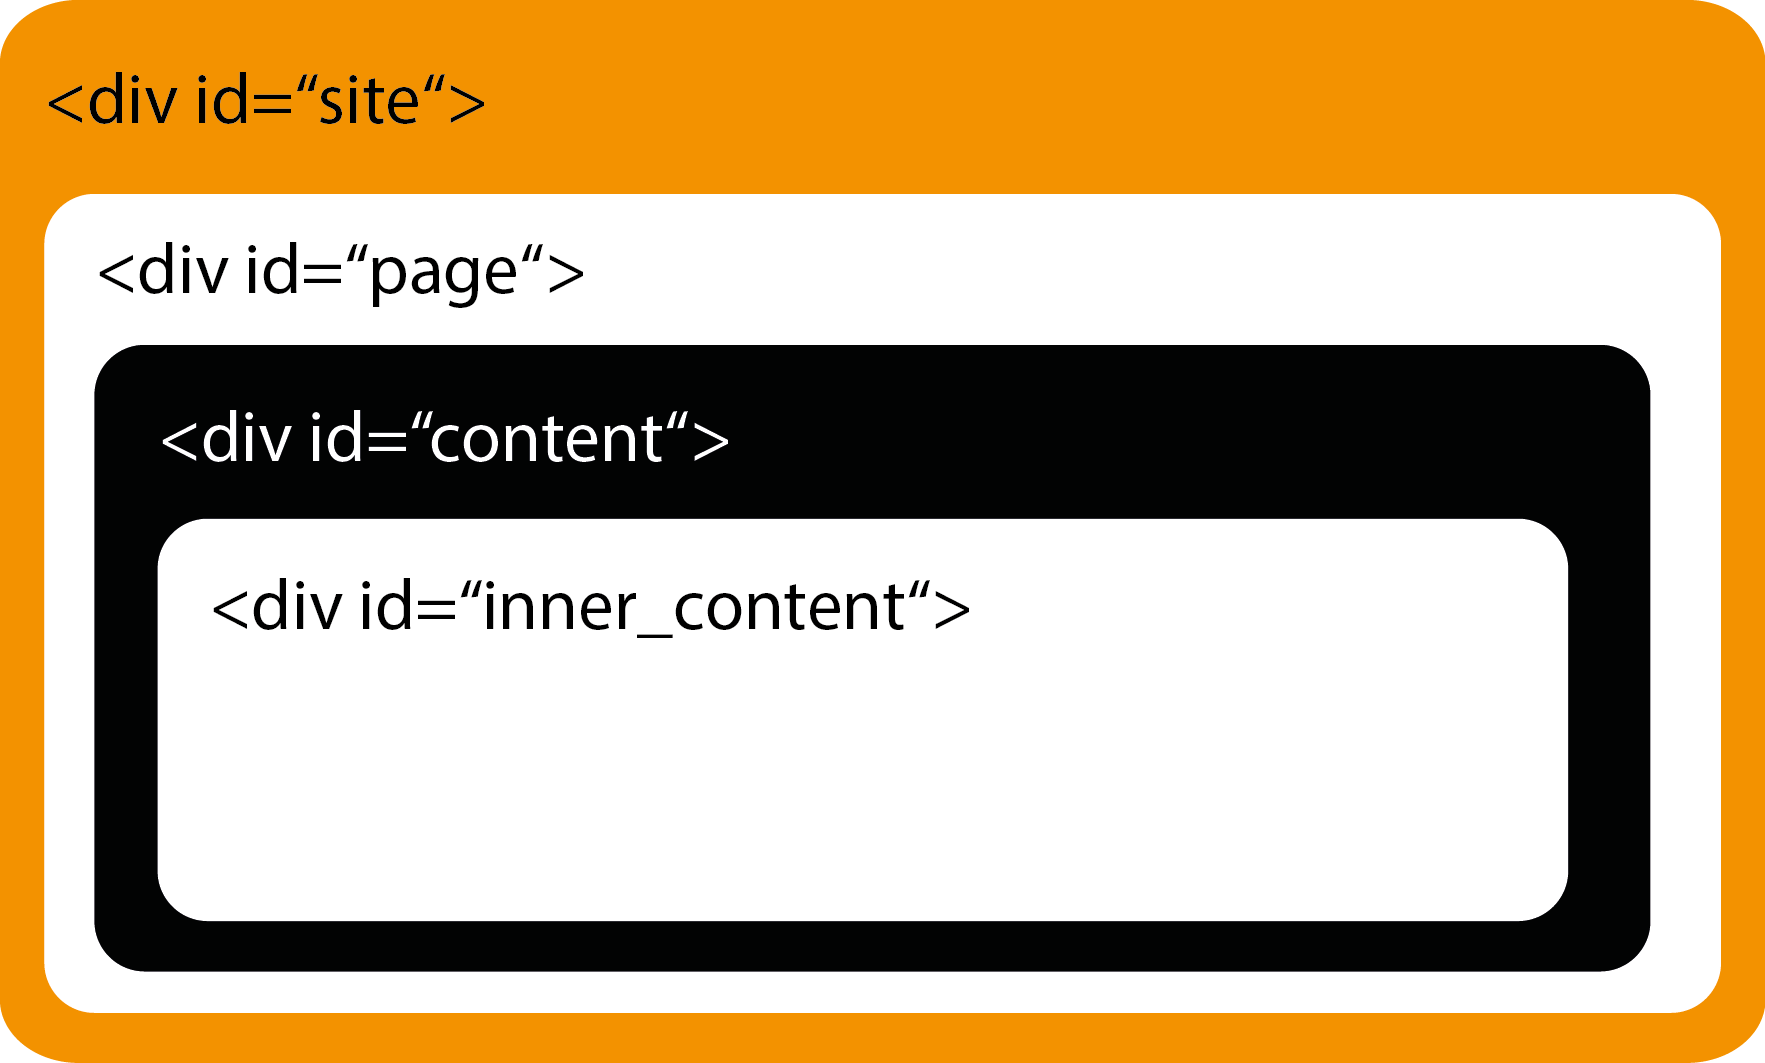
\includegraphics[width=13cm]{images/lare_html.png}
\caption[lare_html]{Basic HTML structure of a web application using \lare{}}
\label{fig:lare_html}
\end{figure}

Every \singlePageApplication{} which uses \lare{} has a hierachical namespace structure.
Typically the namespace consists of 4 levels: A site ID, a page ID, a content ID and an inner-content ID.
Every level in the hierarchy has it's counterpart on the website as shown in figure \ref{fig:lare_html}, a container with an ID telling which part of the namespace it belongs to.

After the \lare{} frontend is initialized it hijacks events like clicks on links and enriches the request with the current website's namespace.
A \lare{} backend analyzes the namespace of the requested website and the one sent in the request.
For every hierarchy level it checks if both namespaces match.
If on one level the namespaces don't match the containers according to this level will be responded to the request.
An optimized web application only grabs the data necessary for those containers and render them afterwards.
The \lare{} frontend retrieves the response, replaces the containers at the website and updates the current namespace.

\begin{figure}[H]
\centering

\includegraphics[height=13cm]{images/lare.png}
\caption[lare_components]{Component and communication diagram of \lare{}}
\label{fig:lare_components}
\end{figure}

As shown in fig. \ref{fig:lare_components} the overall structure of \lare{} is similar to normal \ajax{} requests (compare fig. \ref{fig:ajax_components}).
The \ajax{} engine of \lare{} is \lareJS{}.
In addition to \ajax{}, \lare{} has a backend which helps to reduce server load and maps responses to the given namespace.
Optimally this analyzation is done as first action when retrieving a request by the web server.
Backend queries such database queries and such can then by left out if they are not necessary in the current namespace situation.


\subsection{Realization}
To load a page, the first request is a normal \httpRequest{} followed by a JavaScript script initializing the \lare{} frontend module.
Further requests to the same host are then initiated by this module.
The \http{} header of these requests is extended by the namespace of the current website.
The web server using a \lare{} backend compares the namespace of the requested resource and the namespace in the \http{} header.
It then decides which data is needed to be gathered and which template should be used to render those.

The content delivered by the \lare{} backend enriched web server is interpreted by the frontend module and replaces the related containers.
This replacement is implemented using the ID attribute.
Other methods identifying corresponding containers like e.g. X-Path are not as generic in it's position on the page as the ID.

Usage of the History API makes it then possible to update the content and change the URL like it would be made by normal requests.
This is possible with the use of the pushState method introduced in the History API.
Back- and forward-buttons and bookmarks in a browser will work like on a normal request using this function.

Normal \httpRequest{}s and \lare{} requests request the same URL which makes it easy to crawl.
While on normal requests a full \webPage{} is responded \lare{} requests only get the changed containers as response.
Search engines and other crawlers are able to crawl every link it can find on a page and interpret it as normal \webPage{}s without any deficit.

\subsubsection{\lare{} frontend}

A \lare{} frontend has as mentioned before a few things to be implemented.
The first requirement is the ability to hijack page changes.
This can be implemented by e.g. replacing the default event listeners for anchor-tags.
A new event listener then has to implement an enrichment of the HTTP header by the namespace using the \enquote{HTTP-X-LARE} key.
On initial requests the current namespace should be served as an attribute at the <body> tag called data-lare-namespace.
\lare{} requests serve a new namespace as content of a tag <pjaxr-namespace>.

As heart of \lare{} dynamic URL changes have to be implemented after getting the response.
This should be done by using the pushstate function.

The biggest functionality of the \lare{} frontend is the replacement.
A response of a \lare{} request is divided into a <lare-head> tag, a <lare-body> tag and the <lare-namespace> tag.
Elements of the <lare-head> should be a new <title> tag and <meta> tags matching the new content. 
Additionally scripts or styles can be linked in this section when they are needed by the new content.

The <lare-body> tag will contain the new content which should be replace old one.
Each container inside the <lare-body> will be searched by it's ID inside the current page and will then replace it's predecessor.

\subsubsection{\lare{} backend}

A \lare{} backend should first interpret the \enquote{HTTP-X-LARE} item in the HTTP header.
Every layer of the namespace should have it's own name.
As a default naming convention the layers should have the names \emph{site}, \emph{page}, \emph{content}, \emph{inner\_content} from start to the end.
Per layer a variable should save the matching state.
Those variables have to be accessible by views and controllers to give them the possibility to decide which backend requests should be made and which templates should be used.

\subsubsection{\lare{} templating}

To avoid a lot of overhead when using \lare{} a specific templating system is recommended.

A default template for the first request could be like this:

\begin{minipage}[c]{0.95\linewidth}
\begin{lstlisting}
<!Doctype html>
<html>
<head>
  <title></title>
  ...
</head>
<body data-lare-namespace="Lare.Namespace">
  <div id="site">
    ...
  </div>
</body>
</html>
\end{lstlisting}
\end{minipage}

As shown above, it is a normal HTML5 template.
The only specific code you have to write when using \lare{} is the \emph{data-lare-namespace} attribute at the body tag.

The \lare{} template has to be formed like this:

\begin{minipage}[c]{0.95\linewidth}
\begin{lstlisting}
<lare-head>
  <title></title>
  ...
</lare-head>
<lare-body>
  <div id="site">
    ...
    <div id="page">
       ...
    </div>
    ...
  </div>
</lare-body>
<lare-namespace>Lare.Namespace</lare-namespace>
\end{lstlisting}
\end{minipage}

The <lare-head> tag is the conterpart to the <head> tag, <lare-body> to <body>.
Instead of an attribute in the <lare-body> tag, the namespace will be delivered in the <lare-namespace> tag.

For performance improvements it is intended to have a hierarchical structure as seen in fig. \ref{fig:lare_html}.

When e.g. the first namespace matches, the <lare-body> could only deliver the page conatiner:

\begin{minipage}[c]{0.95\linewidth}
\begin{lstlisting}
<lare-body>
  <div id="page">
    ...
  </div>
</lare-body>
<lare-namespace>Lare.AnotherNamespace</lare-namespace>
\end{lstlisting}
\end{minipage}





\newpage{}

\section{Implementation}

Considering object-oriented programming the \emph{Lare} object builds the fundament of a \lare{} backend.
It is a singleton in the request scope.
When receiving a request the server creates it and analyzes the current \http{} header whether a namespace is set or not.
\\
The \lare{} object contains all necessary data and functions.


\subsection{\phpLare{}}
\phpLare{} is a general \lare{} backend to be used in PHP.
It builds the base of every other \lare{} module in PHP, especially for template engines.
\\
As defined before the \lare{} object is implemented as a request-scoped singleton.
This object gets created by the get\_instance() method.
To prevent multiple objects of this class the \_\_clone() and  \_\_construct() methods are replaced by empty functions.
\\
Automatically one object gets instantiated after the definition of this class.


\subsubsection{API}

\large{\textbf{\textit{Lare::is\_enabled()}}}
\\
Returns true if the current request is a Lare request, otherwise false.
\\
\\
\\
\large{\textit{\textbf{Lare::set\_current\_namespace(\$namespace)}}}
\\
\\
\begin{tabular}{|p{4cm}|p{9cm}|}
    \hline
    \textbf{name} & \textbf{description} \\
    \hline
    \$namespace & specifies the namespace which should be set as the current namespace. \\
    \hline
\end{tabular}
\\
\\
Sets the namespace of the current page.
\\
\\
\\
\large{\textbf{\textit{Lare::get\_current\_namespace()}}
\\
Returns the namespace of the current request.
\\
\\
\\
\large{\textbf{\textit{Lare::get\_matching\_count(\$extension\_namespace=None)}}}
\\
\begin{tabular}{|p{4cm}|p{8cm}|}
    \hline
    \textbf{name} & \textbf{description} \\
    \hline
    \$extension\_namespace & (optional) specifies the namespace which should be matched. If not set the current namespace of the Lare object will be used instead. \\
    \hline
\end{tabular}
\\
\\
Returns how many parts of the \$extension\_namespace and the previous namespace (from outer to inner) are matching, before the first mismatch occurs.
\\
\\
\\
\large{\textbf{\textit{Lare::matches(\$extension\_namespace=None)}}}}
\\
\begin{tabular}{|p{5cm}|p{8cm}|}
    \hline
    \textbf{name} & \textbf{description} \\
    \hline
    \$extension\_namespace & (optional) specifies the namespace which should be matched. If not set the current namespace of the Lare object will be used instead. \\
    \hline
\end{tabular}
\\
\\
Returns true if the extension\_namespace matches the previous namespace (on as many layers as extension\_namespace has), otherwise false.
\\
\\
\\
\large{\textbf{\textit{Lare::get\_instance()}}}
\\
Returns the \lare{} singleton and creates it if not instantiated before.

\subsection{\twigLare{}}
Twig-Lare brings Lare functionality to the template engine Twig\footnote{http://twig.sensiolabs.org/}.
Twig is used by Symfony, a framework which is used in e.g. Drupal 8, eZPublish, phpBB and Sylius.
\\
Twig-Lare is implemented as a Twig extension.
It consists of a TwigTokenParser and the global variable lare\_current\_namespace.
The TwigTokenParser
\\
Twig\_Lare\_TokenParser\_LareExtends is the heart of the extension.
It provides the possibility to use the tag \{\% lare\_extends \%\} in the way the default twig tag \{\% extends \%\} tag is used.
Additionally it prevents multiple extend tags.
Furthermore it is ensured that it is not called inside a block tag, like seen in the default twig tag.

\begin{minipage}[c]{0.95\linewidth}
\begin{lstlisting}[caption=Example Lare Template, label=example_lare_template]


  <div id="page">
    ...
  </div>


  {{ current_lare_namespace }}

\end{lstlisting}
\end{minipage}
\\
Listing \ref{example_lare_template} shows the usage of this tag.
Using Symfony \enquote{::} is a shortcut for the default template directory.
When the current namespace is not inside \emph{Lare.Namespace} it extends to the base.twig template, because the second namespace does not match then.
When the current namespace is \emph{Lare.Namespace} lare.twig will get extended.
\\
As the namespace matching occurs on the second level in this example, the overridden block should be the according one.
For the naming in this thesis the \emph{page} block should be provided.
Inside this block a <div> container with the according ID has to be placed.

\subsubsection{API}

\large{\textbf{\textit{\{\% lare\_extends \$default\_template \$lare\_namespace \$lare\_template \%\}}}}
\\
\begin{tabular}{|p{4cm}|p{8cm}|}
    \hline
    \textbf{name} & \textbf{description} \\
    \hline
    \$default\_template & specifies which template should be extended in case of a non matching namespace. \\
    \hline
    \$lare\_namespace & (optional) specifies the namespace which is tested against to decide whether the \$default\_template or the \$lare\_template should be extended. If not set, \$default\_template will be extended. \\
    \hline
    \$lare\_template & (optional, default='::\_\_lare.html') specifies which template should be extended in case of a namespace match. \\
    \hline
\end{tabular}

Extends the \$default\_template if \$lare\_namespace is not matching, extends \$lare\_template otherwise.


\subsection{\djangoLare{}}

\djangoLare{} was the first backend of \lare{}.
It was introduced as a single object containing logic and template tools.
After implementing \phpLare{} we decided to change the structure of the django backend towards the new segmentation.
\\
Similar to the combination of \phpLare{} and \twigLare{}, \djangoLare{} consists of a Lare object as in the PHP backend and implements the same templating tools as the Twig extension.
Still as one package it is available via \emph{pip install django-lare} command.


\subsubsection{API}
The \textbf{lare\_extends} tag should be used in the django templating engine.

\newpage{}
\noindent{}\large{\textbf{\textit{\{\% lare\_extends default\_template lare\_namespace lare\_template \%\}}}}
\\
\\
\begin{tabular}{|p{4cm}|p{9cm}|}
    \hline
    \textbf{name} & \textbf{description} \\
    \hline
    default\_template & specifies which template should be extended in case of a non matching namespace. \\
    \hline
    lare\_namespace & (optional) specifies the namespace which is tested against to decide whether the default\_template or the lare\_template should be extended. If not set, default\_template will be extended. \\
    \hline
    lare\_template & (optional, default='\_\_lare.html') specifies which template should be extended in case of a namespace match. \\
    \hline
\end{tabular}
\\
\\
\\
Extends the default\_template if lare\_namespace is not matching, extends lare\_template otherwise.
\\
\\
\\
\\
In the following API documentation of the \textbf{\lare{}} object will \textbf{lare} represent the singleton instance.
\\
\\
\\
\large{\textbf{\textit{lare.is\_enabled()}}}
\\
Returns true if the current request is a Lare request, otherwise false.
\\
\\
\\
\large{\textit{\textbf{lare.set\_current\_namespace(namespace)}}}
\\
\\
\begin{tabular}{|p{4cm}|p{9cm}|}
    \hline
    \textbf{name} & \textbf{description} \\
    \hline
    namespace & specifies the namespace which should be set as the current namespace. \\
    \hline
\end{tabular}
\\
\\
Sets the namespace of the current page.
\\
\\
\\
\large{\textbf{\textit{lare.get\_current\_namespace()}}
\\
Returns the namespace of the current request.
\\
\\
\\
\large{\textbf{\textit{lare.get\_matching\_count(extension\_namespace=None)}}}
\\
\begin{tabular}{|p{4cm}|p{8cm}|}
    \hline
    \textbf{name} & \textbf{description} \\
    \hline
    extension\_namespace & (optional) specifies the namespace which should be matched. If not set the current namespace of the Lare object will be used instead. \\
    \hline
\end{tabular}
\\
\\
Returns how many parts of the extension\_namespace and the previous namespace (from outer to inner) are matching, before the first mismatch occurs.
\\
\\
\\
\large{\textbf{\textit{lare.matches(extension\_namespace=None)}}}}
\\
\begin{tabular}{|p{4cm}|p{8cm}|}
    \hline
    \textbf{name} & \textbf{description} \\
    \hline
    extension\_namespace & (optional) specifies the namespace which should be matched. If not set the current namespace of the Lare object will be used instead. \\
    \hline
\end{tabular}
\\
\\
Returns true if the extension\_namespace matches the previous namespace (on as many layers as extension\_namespace has), otherwise false.
\\
\\
\\
\large{\textbf{\textit{lare.get\_instance()}}}
\\
Returns the \lare{} singleton and creates it if not instantiated before.
\\
\\
\\
After modifications and restructuring of \djangoLare{} the API is similar to the API of \phpLare{}.


\subsection{\lareJS{}}
\lareJS{}, as successor of jquery-pjaxr, is the JavaScript frontend engine for \lare{}, using AJAX to communicate with the server.
It was first built as an extended version of jquery-pjax, allowing to replace multiple containers with one request, instead of only one.
Other than in jquery-pjax it is not needed to define which containers should be replace in the frontend.
It is the job of the backend to define which elements should change, as the frontend does an ID based matching.
\lareJS{} additionally provides the functionality to extend the HTTP header by the current \lare{} namespace.
\\
After the script is loaded it automatically tests if the History API is available or not.
If the requirements are fulfilled it gets initialized.
\\
As described in \ref{lare_frontend} a \lare{} frontend has to hijack page changes.
\lareJS{}, implemented as a jQuery\footnote{\url{https://jquery.com}} plugin realizes this by just one function call, e.g. \$(document).lare('a');.
jQuery plugins normally have a syntax like \$('a').lare();.
But semantically \lareJS{} sets the focus on the engine itself, instead of the items.
Anyway the event listeners will be set by using this method.
\\
Besides the \lare{} functionality \lareJS{} provides utilities for JavaScript including helping functions like e.g. \$(document).lareAlways(function(e) { ... });.
This runs function(e) {} every time a lare request is finished successfully or a history step is made.
This makes it possible to imitate \$(document).ready(function(e) { ... }); provided by jQuery, to hook functions to the document ready event.

\newpage{}

\section{Evaluation}
\todo{describe test design}
\lare{} is tested based on a sample web application.
It provides different type of sites which are designed to perform the different aspects of this evaluation.

%As stated in \cite{bib:palomaeki09} \enquote{proper test definition, execution, reporting and repeatable test results are of utmost importance}.

To evaluate \lare{} we first test it's functionality.
We check if the desired content is delivered and if \lare{} is actually performing like expected.

It is not easy to test \ajax{} \webApplication{}s.
As seen in \cite{bib:marchetto_tonella_ricca07} there is a lack of good testing tools, especially when it comes to white-box testing.
\selenium{} is mentioned there as a good tool for black-box testing.
It is also suggested in \cite{bib:palomaeki09} for a non-abstract HTTP request performance testing, which can represent the requests of a single user.

In \cite{bib:marchetto_tonella_ricca08} a new automated testing technique is introduced, again based on \selenium{}.

As to evaluate \lare{} there is no need to actually test the whole application, but only to check whether \lare{} works, \selenium{} in our case is sufficient.

We make specific requests and want an specific answer of it.
Especially we want to have the same content rendered through \lare{} as through normal \httpRequest{}s.

\selenium{} additionally makes it possible to use different \webdriver{}s, in this thesis FireFox and Chrome are used.
This is important because of the different implementations of browsers' features.

To test the performance, we will use two technologies.
\cite{bib:bozdag_mesbah_vanDeursen08}
First of all \curl{} based tests will be done.
Those tests will focus on the first response, containing the markup.
This will show how \lare{} influences the webserver.

Additionially the webapp will be benchmarked by using the Chrome Network Tools.
This method provides the possiblity to check whether further requests for scripts, images, etc. are influenced.
The Chrome Network Tools will show the actual load time the user has to wait for, until the whole page is loaded.

To make the tests as representive as possible caching in the relevant layers will be enabled and disabled if to see whether it influences the results or not.
Some caching algorithms can not be easily disabled.
E.g. hardware and hard drive caching will not be disabled in our tests.
As those caching algorithms will not effect the results much, we let them enabled.

Mysql's caching method Query Caching will be enabled and disabled.
Twig, the template engine allows caching, which will be enabled and disabled as well.
Additionally all tests are performed on a local machine and a remote server, to see whether the latency takes effect in the performance of \lare{}.

We will distinguish between static pages without database queries and dynamic pages which have those.
Every page relevant for the test will be requested in different modes.
First of all every site will be requested normally.
After that it will be requested with \lare{} enabled.
As \lare{} should only influence subsequent requests, every page will be tested with \http{} headers from different sources, imitating those requests.

%As one traditional testing model, we will evaluate the \pjaxr{} sample application via blackbox tests.
%Testing \ajax{} is not trivial due to multiple programming- and markup-languages influencing it. 
%One possibility to test web applications, as suggested in \cite{bib:lundmark11}, is Selenium\footnote{http://www.seleniumhq.org/}.
%With this tool it is possible to generate automated tests for web applications.
%
%To evaluate whether the application is crawlable or not is an important criteria whether \pjaxr{} fulfills it goals.
%Finding all the content delivered in all different URLs in the sitemap should be the target to acquire.
%The crawled content should be similar to a non-dynamic HTML file, defined for every URL.
%Content which is not directly provided via an URL but asynchronously, like via an autocompletion, should not be relevant.
%
%One way to crawl \ajax{} web applications, recommended in \cite{bib:crawljax_tweb12} is to use Crawljax\footnote{http://crawljax.com/}. 
%It explores \ajax{}-based web applications by following every link recursively and saving the associated content. In this thesis the three endpoints of the sample project will be crawled by Crawljax to see whether all endpoints provide the same content or not.
%
%Another way to evaluate whether \pjaxr{} fulfils its goals, is testing if the Googlebot\footnote{http://google.com/bot.html} will discover all the content provided.
%Again, all three endpoints will be tested to check, if all data is found by this technique.
%While Crawljax is intended to find not easily accessible content, Googlebot is intended to find content, matching design patterns\footnote{https://developers.google.com/webmasters/ajax-crawling/} by Google. This fact makes it more challenging for \pjaxr{}, not implementing these, to have good results in this test.


\subsection{Sample web application}

The sample web application used to test \lare{} in this thesis is implemented in PHP.
To implement \lare{} we used \lareJS{} in the frontend, \twigLare{} and \phpLare{} for the backend.

We use the MVC design pattern, but with a slightly different naming.
For web applications it is common to use the name \emph{template} for what is called view in the MVC.
As "controller" is not a common name PHP web applications as well, we use the phrase \emph{view} for those.
With this we follow the naming of django\footnote{https://docs.djangoproject.com/en/1.8/faq/general/\#django-appears-to-be-a-mvc-framework-but-you-call-the-controller-the-view-and-the-view-the-template-how-come-you-don-t-use-the-standard-names}.

Instead of using models for this benchmark evaluation, we are using raw SQL queries to ensure the same queries are made every time.
Nevertheless it is prepared to inherit from the BaseModel class to be create models for later presentation purposes.

The sample web application consists of 2 static pages \emph{/home/} and \emph{/imprint/}.

To demonstrate dynamic \WebPage{}s we used the Delicious Dataset\footnote{http://fabianabel.de/data/mypes-www2010.html}.
This is available under \emph{/tags/}.

On the left side is a list to sub pages where the tags are categorized by it's starting character.
Per alphabetic character one of those pages exists, additionally one page for tags starting with numbers and one starting with non alphanumeric characters.
Behind each \emph{category} the count of tags in this category is displayed.
This list is available on every sub page under the \emph{/tags/} url.

On the right side a paginated list of all distinct tags in the current category is shown.
It is sorted alphabetically and 30 tags per page are displayed.

We are using the namespaces like shown in tab. \ref{tab:sampleapp_namespaces}.

\begin{table}[h]
\centering
\begin{tabular}{llll}
	\hline
	\textbf{URL} & \textbf{Site} & \textbf{Page} & \textbf{Content} \\
	\hline
	/ & Lare & Home &  \\
	/imprint/ & Lare & Imprint &  \\
	/tags/ & Lare & Tags & all \\
	/tags/a/ & Lare & Tags & a \\
	/tags/.../ & Lare & Tags & ... \\
	\hline
\end{tabular}
\caption{Namespaces of the sample web application}
\label{tab:sampleapp_namespaces}
\end{table}


\subsection{Tests}

To test the performance of \lare{} a few different types of requests are needed to benchmark.
The reference level will be a normal \httpRequest{} to each \webPage{}.

The tested pages are available at the URLs:

\begin{itemize}
\item /
\item /imprint/
\item /tags/p/
\item /tags/p/2/
\end{itemize}

Additionally the \webPage{}s will be requested via \lare{}.
To achieve this at \curl{} we extend the request's header with the corresponding \emph{HTTP-X-LARE} namespace.

With \selenium{} we will later test the pages with real web browsers to get results which are closer to reality.
The tested page to page requests are:

\begin{itemize}
  \item Self:
    \begin{itemize}
      \item / to /
      \item /imprint/ to /imprint/
      \item /tags/p/ to /tags/p/
      \item /tags/p/2/ to /tags/p/2/
    \end{itemize}
  \item Static page matching Site-Namespace:
    \begin{itemize}
      \item / to /imprint/
      \item /imprint to /
    \end{itemize}
  \item Dynamic page matching Site-Namespace:
    \begin{itemize}
      \item / to /tags/p/
      \item /imprint/ to /tags/p/
    \end{itemize}
  \item Dynamic page to static page:
    \begin{itemize}
      \item /tags/p/ to /
      \item /tags/p/2/ to /
      \item /tags/p/ to /imprint/
      \item /tags/p/2/ to /imprint/
    \end{itemize}
  \item Dynamic page matching Page-Namespace:
    \begin{itemize}
      \item /tags/p/ to /tags/p/2/
      \item /tags/p/2/ to /tags/p/
    \end{itemize}
\end{itemize}

\subsection{\curl{}\label{curl}}
\todo{curl usage of test design}
We are using \curl{} to test the plain load times of the initial request of normal \httpRequest{}s and \lare{} requests.
Those \curl{} requests do not include additional data like images, scripts and stylesheets, just the plain HTML.

The bash script \enquote{curl\_tests.sh} provides the functionality to run those \curl{} tests.
To use it run 
\enquote{/.../evaluation/curl/curl\_tests.sh URL MAX\_RUNS LARE\_NAMESPACE CACERT}.

URL dedicates where the web application is available, e.g. \emph{http://lare.iekadou.com}, MAX\_RUNS defines how many \curl{} requests per page should be made.
LARE\_NAMEPSACE defines the namespace, which should be used when testing the \lare{} requests, e.g. Lare.Tags.p.
CACERT is the only optional paremeter, which should only be set when requesting an SSL server. It then should be the path to the CACERT file.


To test all relevant sites we defined a variable PAGES inside the script, containing URLs \emph{/}, \emph{/imprint/}, \emph{/tags/p/} and \emph{/tags/p/2/}.
For each page of those we make a normal request, followed by a \lare{} request, with the namespace defined in LARE\_NAMESPACE. 
To get better test results we repeat those two requests \emph{MAX\_RUN} times. The output represents then the load times needed in seconds.

For the results in this thesis, markes as local, we use a Macbook Pro Retina Early 2013 (2,7 GHz, 16GB Ram).
As web server we are running an Apache via Mamp Pro 3.1 for Mac OSX with PHP 5.3.6.
As database server we are using MySQL in version 5.5.42.

When running the benchmarks on an external server we are using a virtual server running OS: Ubuntu 12.04.5 LTS.
It has a Intel(R) Xeon(R)CPU E5520, 4 GB ram, PSA version 11.5.30, Mysql version 5.5.41 and php version 5.3.10.

Additionally we test every request with database caching (DBC) enabled, disabled and template caching(TC) enabled and disabled.

\subsubsection{Results}

You can see the full results of our benchmarks in tables \ref{tab:curl_results_local} and \ref{tab:curl_results_external}.

First we will take a look at the results of the local tests.

Those tests show that the load times of \lare{} requests of static pages in general are quite the same then on normal \httpRequest{}s.
\lare{} does not seem to have a huge effect on static pages without a lot of heavy operations like backend queries. It makes the responses a bit smaller, but no logical operations can be avoided.

Template caching has not a big effect on the difference between \lare{} and normal requests, but the absolute load times get a bit down.
Database caching has not even on the absolute times an effect at those static pages, because no backend queries are made.

When requesting a dynamic page and sending the namespace of a static page like in our tests \enquote{Lare.Tags.Imprint} the results of \lare{} are still similar to normal requests.
This can be explained by the fact that almost the whole page needs to be changed, including every database query.

The results on dynamic pages with a related namespace, in our case \enquote{Lare.Tags.p} differ a lot.
When database caching is enabled the load times of \lare{} are around 90\% with template caching enabled and about 80\% of the normal load times with disabled template caching.

Without database caching this these times they are \textbf{7\%} with template caching and \textbf{10\%} without.

Those improvemnts are caused by the amount of database queries that can be avoided. This also explains the differences between enabled and disabled database caching settings.

When we take a look at the external tests we can see the same pattern.
The effect of \lare{} on dynamic pages is a bit smaller.
Wihtout database caching they are about \textbf{12\%} with template caching and \textbf{16\%} without.

Why does it have not this huge effect anymore?

This can be explained with the latency.
In our tests it was 40ms.
\httpRequest{}s need two Round Trip Times, or four times the latency for connection establishment.
When we substract those 160ms from the normal and the \lare{} requests we see ratios similar to the local tests.

In general we can say, that \lare{} has more effect the more time of backend logic like database queries can be avoided.

\newpage{}

\begin{center}
\begin{longtable}{llllll}
	\hline
	\textbf{URL} & \textbf{Normal loadtime} & \textbf{\lare{} loadtime} & \textbf{Namespace} & \textbf{TC} & \textbf{DBC} \\
	\hline
	/ & 0.03740 & 0.03600 (96,26\%) & Lare.Tags.p & + & + \\
	/imprint/ & 0.03590 & 0.03620 (100,84\%) & Lare.Tags.p & + & + \\
	/tags/p/ & 0.03950 & 0.03480 (88,10\%) & Lare.Tags.p & + & + \\
	/tags/p/2/ & 0.03940 & 0.03550 (90,10\%) & Lare.Tags.p & + & + \\
	\hline
	/ & 0.03370 & 0.03610 (107,12\%) & Lare.Tags.Imprint & + & + \\
	/imprint/ & 0.03570 & 0.03450 (96,64\%) & Lare.Tags.Imprint & + & + \\
	/tags/p/ & 0.03910 & 0.04080 (104,36\%) & Lare.Tags.Imprint & + & + \\
	/tags/p/2/ & 0.04040 & 0.03960 (98,02\%) & Lare.Tags.Imprint & + & + \\
	\hline
	\hline
	/ & 0.03400 & 0.03380 (99,41\%) & Lare.Tags.p & + & - \\
	/imprint/ & 0.03430 & 0.03480 (101,46\%) & Lare.Tags.p & + & - \\
	\textbf{/tags/p/} & \textbf{1.02180} & \textbf{0.07230 (7,08\%)} & \textbf{Lare.Tags.p} & \textbf{+} & \textbf{-}\\
	/tags/p/2/ & 1.03130 & 0.07310 (7,09\%) & Lare.Tags.p & + & - \\
	\hline
	/ & 0.03440 & 0.03650 (106,10\%) & Lare.Tags.Imprint & + & - \\
	/imprint/ & 0.03540 & 0.03480 (98,31\%) & Lare.Tags.Imprint & + & - \\
	/tags/p/ & 1.02390 & 1.04130 (101,70\%) & Lare.Tags.Imprint & + & - \\
    \textbf{/tags/p/2/} & \textbf{1.03440} & \textbf{1.04980 (101,49\%)} & \textbf{Lare.Tags.Imprint} & \textbf{+} & \textbf{-}\\
    \hline
	\hline
	/ & 0.07210 & 0.06660 (92,37\%) & Lare.Tags.p & - & - \\
	/imprint/ & 0.06690 & 0.06410 (95,81\%) & Lare.Tags.p & - & - \\
	/tags/p/ & 1.08420 & 0.10720 (9,89\%) & Lare.Tags.p & - & - \\
    \textbf{/tags/p/2/} & \textbf{1.09660} & \textbf{0.10900 (9,94\%)} & \textbf{Lare.Tags.p} & \textbf{-} & \textbf{-}\\
    \hline
	/ & 0.06920 & 0.06860 (99,13\%) & Lare.Tags.Imprint & - & - \\
	/imprint/ & 0.06840 & 0.06520 (95,32\%) & Lare.Tags.Imprint & - & - \\
	/tags/p/ & 1.09020 & 1.09620 (100,55\%) & Lare.Tags.Imprint & - & - \\
	/tags/p/2/ & 1.09000 & 1.07740 (98,84\%) & Lare.Tags.Imprint & - & - \\
	\hline
	\hline
	/ & 0.07070 & 0.06630 (93,78\%) & Lare.Tags.p & - & + \\
	/imprint/ & 0.06710 & 0.06510 (97,02\%) & Lare.Tags.p & - & + \\
	/tags/p/ & 0.08440 & 0.06990 (82,82\%) & Lare.Tags.p & - & + \\
	/tags/p/2/ & 0.08550 & 0.06930 (81,05\%) & Lare.Tags.p & - & + \\
	\hline
	/ & 0.07010 & 0.06790 (96,86\%) & Lare.Tags.Imprint & - & + \\
	/imprint/ & 0.06770 & 0.06510 (96,16\%) & Lare.Tags.Imprint & - & + \\
	/tags/p/ & 0.08540 & 0.08230 (96,37\%) & Lare.Tags.Imprint & - & + \\
	\textbf{/tags/p/2/} & \textbf{0.08390} & \textbf{0.08220 (97,97\%)} & \textbf{Lare.Tags.Imprint} & \textbf{-} & \textbf{+} \\
	\hline
\caption{\curl{} results on a local machine}
\label{tab:curl_results_local}
\end{longtable}
\end{center}



\begin{center}
\begin{longtable}{llllll}
	\hline
	\textbf{URL} & \textbf{Normal loadtime} & \textbf{\lare{} loadtime} & \textbf{Namespace} & \textbf{TC} & \textbf{DBC} \\
	\hline
	/ & 0.16520 & 0.14070 (85,17\%) & Lare.Tags.p & + & + \\
	/imprint/ & 0.14360 & 0.12850 (89,48\%) & Lare.Tags.p & + & + \\
	/tags/p/ & 0.15420 & 0.13180 (85,47\%) & Lare.Tags.p & + & + \\
	/tags/p/2/ & 0.14610 & 0.14200 (97,19\%) & Lare.Tags.p & + & + \\
	\hline
	/ & 0.14050 & 0.13350 (95,02\%) & Lare.Tags.Imprint & + & + \\
	/imprint/ & 0.13690 & 0.13630 (99,56\%) & Lare.Tags.Imprint & + & + \\
	/tags/p/ & 0.14470 & 0.14170 (97,93\%) & Lare.Tags.Imprint & + & + \\
	/tags/p/2/ & 0.14230 & 0.13310 (93,53\%) & Lare.Tags.Imprint & + & + \\
	\hline
	\hline
	/ & 0.14860 & 0.14580 (98,11\%) & Lare.Tags.p & + & - \\
	/imprint/ & 0.14990 & 0.13830 (92,66\%) & Lare.Tags.p & + & - \\
	\textbf{/tags/p/} & \textbf{1.55500} & \textbf{0.19070 (12,26\%)} & \textbf{Lare.Tags.p} & \textbf{+} & \textbf{-} \\
	/tags/p/2/ & 1.52150 & 0.19600 (12,88\%) & Lare.Tags.p & + & - \\
	\hline
	/ & 0.14160 & 0.14080 (99,44\%) & Lare.Tags.Imprint & + & - \\
	/imprint/ & 0.14300 & 0.13790 (96,43\%) & Lare.Tags.Imprint & + & - \\
	/tags/p/ & 1.50930 & 1.54400 (102,30\%) & Lare.Tags.Imprint & + & - \\
	\textbf{/tags/p/2/} & \textbf{1.51030} & \textbf{1.56460 (103,59\%)} & \textbf{Lare.Tags.Imprint} & \textbf{+} & \textbf{-} \\
	\hline
	\hline
	/ & 0.20450 & 0.18600 (90,95\%) & Lare.Tags.p & - & - \\
	/imprint/ & 0.20350 & 0.18130 (89,09\%) & Lare.Tags.p & - & - \\
	/tags/p/ & 1.64180 & 0.30550 (18,61\%) & Lare.Tags.p & - & - \\
	\textbf{/tags/p/2/} & \textbf{1.65950} & \textbf{0.24830 (14,96\%)} & \textbf{Lare.Tags.p} & \textbf{-} & \textbf{-} \\
	\hline
	/ & 0.20390 & 0.19800 (97,11\%) & Lare.Tags.Imprint & - & - \\
	/imprint/ & 0.20440 & 0.18360 (89,82\%) & Lare.Tags.Imprint & - & - \\
	/tags/p/ & 1.64260 & 1.62680 (99,04\%) & Lare.Tags.Imprint & - & - \\
	/tags/p/2/ & 1.63810 & 1.67440 (102,22\%) & Lare.Tags.Imprint & - & - \\
	\hline
	\hline
	/ & 0.20940 & 0.20020 (95,61\%) & Lare.Tags.p & - & + \\
	/imprint/ & 0.20300 & 0.19040 (93,79\%) & Lare.Tags.p & - & + \\
	/tags/p/ & 0.22250 & 0.20760 (93,30\%) & Lare.Tags.p & - & + \\
	/tags/p/2/ & 0.20940 & 0.20160 (96,28\%) & Lare.Tags.p & - & + \\
	\hline
	/ & 0.20800 & 0.20500 (98,56\%) & Lare.Tags.Imprint & - & + \\
	/imprint/ & 0.19970 & 0.19480 (97,55\%) & Lare.Tags.Imprint & - & + \\
	/tags/p/ & 0.21420 & 0.20200 (94,30\%) & Lare.Tags.Imprint & - & + \\
	\textbf{/tags/p/2/} & \textbf{0.21630} & \textbf{0.22510 (104,07\%)} & \textbf{Lare.Tags.Imprint} & \textbf{-} & \textbf{+} \\
	\hline
\caption{\curl{} results on a external machine}
\label{tab:curl_results_external}
\end{longtable}
\end{center}

\subsection{\selenium{}\label{selenium}}

\todo{\selenium{} usage of test design}
To benchmark full page loads including all resources we are using \selenium{}.
This \emph{record and play} tool builds an interface for a usage of multiple \webdriver{}s.
Those \webdriver{}s are provided by most modern browsers like Chrome and Firefox.
For the results in this thesis we used the Firefox \webdriver{}.

We request a page via a normal \httpRequest{} first.
Afterwards we request the same page again via \lare{}.
We are using a lot of different page to page requests, to see where \lare{} has a bigger or smaller effect on the load times.

Like in \ref{curl} we test every page on a local server and an external webserver and we disabled and enable database and template caching.

\subsubsection{Results}

The results of the \selenium{} \webdriver{} tests are different to the ones made with \curl{}.

We first will take a look at the local tests again.
Other than in the \curl{} test results we see a huge effect of \lare{} even on the static pages.
An average \lare{} load time of about 35\% with disabled template caching and 9\% with enabled template caching of the normal load time can be seen here.   2
Other than on a normal request, the browser does not need to load the resources like images, scripts and styles.
This means \lare{} requests often only need one request to make a page change.
A normal requests needs to load, or at least compare, about 9 resources for the same action.

Again requesting a static page does not show any changes when it comes to database caching.

When it comes to dynamic pages we have to take a more detailed look to the requests.
Requesting a dynamic page from another \lare{} namespace with disabled database caching takes almost the same time like a normal request.
This is because the same backend requests need to be done.
Those uncached database requests take as we can see in table \ref{tab:curl_results_local} the majority of time.

With disabled caching in the database and in a related namespace instead, \lare{} has a huge effect.
Enabled template caching improving the load times from 5\% with a disabled template caching to 3,5\%.

When requesting the same pages with enabled database caching we see a \lare{} load time of about 16\% with unrelated namespaces.
Related namespaces in the same configuration lead to values of about 10\%.

Enabled template caching lower the load times of the normal and \lare{} requests, but not of the resources.
This makes \lare{} more effective, because the load times relative to the normal requests incl. all resources decrease.


\begin{center}
\begin{longtable}{llllll}
	\hline
	\textbf{From} & \textbf{To} & \textbf{Normal loadtime} & \textbf{\lare{} loadtime} & \textbf{TC} & \textbf{DBC} \\
	\hline
	/tags/p/ & /tags/p/2/ & 60.0648983ms & 7.3076173ms (12.17\%) & + & + \\
	/tags/p/2/ & /tags/p/ & 51.5302378ms & 5.7457083ms (11.15\%) & + & + \\
	\hline
	/tags/p/ & / & 58.0190003ms & 5.2543307ms (9.06\%) & + & + \\
	/tags/p/2/ & / & 45.1883941ms & 4.159042ms (9.20\%) & + & + \\
	/tags/p/ & /imprint/ & 46.8359346ms & 4.3459044ms (9.28\%) & + & + \\
	/tags/p/2/ & /imprint/ & 47.1970978ms & 4.2372439ms (8.98\%) & + & + \\
	\hline
	/ & / & 56.6017328ms & 5.4929997ms (9.70\%) & + & + \\
	/imprint/ & /imprint/ & 43.3243723ms & 4.1624412ms (76.67\%) & + & + \\
	/tags/p/ & /tags/p/ & 54.4607062ms & 5.5379726ms (10.17\%) & + & + \\
	/tags/p/2/ & /tags/p/2/ & 52.5258287ms & 5.7707781ms (10.99\%) & + & + \\
	\hline
	/ & /tags/p/ & 66.8794388ms & 10.4380685ms (15.61\%) & + & + \\
	/imprint/ & /tags/p/ & 52.089504ms & 9.1059678ms (17.48\%) & + & + \\
	\hline
	/ & /imprint/ & 57.6817111ms & 5.884066ms (10.20\%) & + & + \\
	/imprint/ & / & 45.9628159ms & 4.6333061ms (10.08\%) & + & + \\
	\hline
	\hline
	/tags/p/ & /tags/p/2/ & 1243.4891679ms & 46.5173918ms (3.74\%) & + & - \\
	/tags/p/2/ & /tags/p/ & 1236.3124832ms & 43.4368424ms (3.51\%) & + & - \\
	\hline
	/tags/p/ & / & 53.4060902ms & 5.1304958ms (9.61\%) & + & - \\
	/tags/p/2/ & / & 45.4183183ms & 4.206772ms (9.26\%) & + & - \\
	/tags/p/ & /imprint/ & 46.2665835ms & 4.175386ms (9.02\%) & + & - \\
	/tags/p/2/ & /imprint/ & 46.0661066ms & 4.2264232ms (9.17\%) & + & - \\
	\hline
	/ & / & 53.5617939ms & 5.4352539ms (10.15\%) & + & - \\
	/imprint/ & /imprint/ & 45.0215085ms & 4.4406ms (65.68\%) & + & - \\
	/tags/p/ & /tags/p/ & 1234.5362779ms & 44.369364ms (3.59\%) & + & - \\
	/tags/p/2/ & /tags/p/2/ & 1235.7906042ms & 45.1390014ms (3.65\%) & + & - \\
	\hline
	/ & /tags/p/ & 1246.2746233ms & 1197.6706971ms (96.10\%) & + & - \\
	/imprint/ & /tags/p/ & 1231.1385665ms & 1191.9845789ms (96.82\%) & + & - \\
	\hline
	/ & /imprint/ & 49.8334108ms & 6.1112746ms (12.26\%) & + & - \\
	/imprint/ & / & 44.540915ms & 4.2382487ms (9.52\%) & + & - \\
	\hline
	\hline
	/tags/p/ & /tags/p/2/ & 1281.1725193ms & 69.312793ms (5.41\%) & - & - \\
	/tags/p/2/ & /tags/p/ & 1271.3418256ms & 67.1285484ms (5.28\%) & - & - \\
	\hline
	/tags/p/ & / & 81.102332ms & 27.2707205ms (33.63\%) & - & - \\
	/tags/p/2/ & / & 69.681426ms & 25.9004252ms (37.17\%) & - & - \\
	/tags/p/ & /imprint/ & 68.4034544ms & 24.2320953ms (35.43\%) & - & - \\
	/tags/p/2/ & /imprint/ & 66.3318697ms & 23.254195ms (35.06\%) & - & - \\
	\hline
	/ & / & 80.4801214ms & 27.0665394ms (33.63\%) & - & - \\
	/imprint/ & /imprint/ & 66.282428ms & 23.5402204ms (35.52\%) & - & - \\
	/tags/p/ & /tags/p/ & 1277.0515153ms & 67.8621459ms (5.31\%) & - & - \\
	/tags/p/2/ & /tags/p/2/ & 1266.6883795ms & 68.0796981ms (5.37\%) & - & - \\
	\hline
	/ & /tags/p/ & 1274.8229527ms & 1224.9995695ms (96.09\%) & - & - \\
	/imprint/ & /tags/p/ & 1273.1817246ms & 1221.7685327ms (95.96\%) & - & - \\
	\hline
	/ & /imprint/ & 71.5289704ms & 25.8452978ms (36.13\%) & - & - \\
	/imprint/ & / & 70.3443044ms & 26.8150602ms (38.12\%) & - & - \\
	\hline
	\hline
	/tags/p/ & /tags/p/2/ & 96.6278896ms & 31.5540318ms (32.66\%) & - & + \\
	/tags/p/2/ & /tags/p/ & 84.6051469ms & 29.4296049ms (34.78\%) & - & + \\
	\hline
	/tags/p/ & / & 78.0617908ms & 28.0351468ms (35.91\%) & - & + \\
	/tags/p/2/ & / & 70.2056237ms & 26.3221693ms (37.49\%) & - & + \\
	/tags/p/ & /imprint/ & 66.3406013ms & 23.5038ms (35.43\%) & - & + \\
	/tags/p/2/ & /imprint/ & 67.9293146ms & 23.1398233ms (34.06\%) & - & + \\
	\hline
	/ & / & 79.6650023ms & 27.2197206ms (34.17\%) & - & + \\
	/imprint/ & /imprint/ & 65.1834701ms & 23.0573013ms (35.37\%) & - & + \\
	/tags/p/ & /tags/p/ & 89.4712661ms & 29.4440881ms (32.91\%) & - & + \\
	/tags/p/2/ & /tags/p/2/ & 86.7669023ms & 30.3473338ms (34.98\%) & - & + \\
	\hline
	/ & /tags/p/ & 101.7855178ms & 43.100569ms (42.34\%) & - & + \\
	/imprint/ & /tags/p/ & 84.2801923ms & 42.5754955ms (50.52\%) & - & + \\
	\hline
	/ & /imprint/ & 70.6183847ms & 25.6731125ms (36.35\%) & - & + \\
	/imprint/ & / & 69.7824729ms & 25.9579276ms (37.20\%) & - & + \\
	\hline
\caption{\selenium{} benchmark results on a local machine}
\label{tab:selenium_benchmark_results_local}
\end{longtable}
\end{center}

\newpage{}

\begin{center}
\begin{longtable}{llllll}
	\hline
	\textbf{From} & \textbf{To} & \textbf{Normal loadtime} & \textbf{\lare{} loadtime} & \textbf{TC} & \textbf{DBC} \\
	\hline
	/tags/p/ & /tags/p/2/ & 378.7378772ms & 100.0062951ms (26.41\%) & + & + \\
	/tags/p/2/ & /tags/p/ & 149.1767846ms & 100.5256257ms (67.39\%) & + & + \\
	\hline
	/tags/p/ & / & 177.8015667ms & 101.0766767ms (56.86\%) & + & + \\
	/tags/p/2/ & / & 145.9762462ms & 100.3458274ms (68.74\%) & + & + \\
	/tags/p/ & /imprint/ & 145.1269058ms & 99.0440198ms (68.25\%) & + & + \\
	/tags/p/2/ & /imprint/ & 143.6989026ms & 96.5441573ms (67.19\%) & + & + \\
	\hline
	/ & / & 184.0143055ms & 96.8061586ms (52.61\%) & + & + \\
	/imprint/ & /imprint/ & 146.1839403ms & 102.3730996ms (70.03\%) & + & + \\
	/tags/p/ & /tags/p/ & 158.4086978ms & 96.0358653ms (60.63\%) & + & + \\
	/tags/p/2/ & /tags/p/2/ & 146.5099972ms & 99.6919812ms (68.04\%) & + & + \\
	\hline
	/ & /tags/p/ & 172.8212049ms & 104.4932832ms (60.46\%) & + & + \\
	/imprint/ & /tags/p/ & 146.4761414ms & 108.3417488ms (73.97\%) & + & + \\
	\hline
	/ & /imprint/ & 154.5478889ms & 99.9289012ms (64.66\%) & + & + \\
	/imprint/ & / & 141.8673753ms & 93.5422212ms (65.94\%) & + & + \\
	\hline
	\hline
	/tags/p/ & /tags/p/2/ & 1759.8420863ms & 165.503113ms (9.40\%) & + & - \\
	/tags/p/2/ & /tags/p/ & 1565.4801458ms & 153.9259203ms (9.83\%) & + & - \\
	\hline
	/tags/p/ & / & 183.7747229ms & 99.9362148ms (54.38\%) & + & - \\
	/tags/p/2/ & / & 142.2313467ms & 113.300735ms (79.66\%) & + & - \\
	/tags/p/ & /imprint/ & 143.6316948ms & 104.1513079ms (72.51\%) & + & - \\
	/tags/p/2/ & /imprint/ & 145.2610703ms & 99.569909ms (68.55\%) & + & - \\
	\hline
	/ & / & 174.5883816ms & 95.7787123ms (54.86\%) & + & - \\
	/imprint/ & /imprint/ & 145.7255202ms & 95.7090602ms (65.68\%) & + & - \\
	/tags/p/ & /tags/p/ & 1526.8233515ms & 147.9105317ms (9.70\%) & + & - \\
	/tags/p/2/ & /tags/p/2/ & 1542.0292612ms & 148.6008572ms (9.64\%) & + & - \\
	\hline
	/ & /tags/p/ & 1587.1344271ms & 1474.1047079ms (92.88\%) & + & - \\
	/imprint/ & /tags/p/ & 1556.204205ms & 1544.0254721ms (99.22\%) & + & - \\
	\hline
	/ & /imprint/ & 154.0036756ms & 98.7195222ms (64.10\%) & + & - \\
	/imprint/ & / & 146.4833535ms & 94.3328383ms (64.40\%) & + & - \\
	\hline
	\hline
	/tags/p/ & /tags/p/2/ & 1668.684526ms & 229.4092215ms (13.75\%) & + & - \\
	/tags/p/2/ & /tags/p/ & 1616.4873064ms & 214.1759213ms (13.25\%) & + & - \\
	\hline
	/tags/p/ & / & 221.7372628ms & 154.6111857ms (69.73\%) & + & - \\
	/tags/p/2/ & / & 196.4610228ms & 161.2432577ms (82.07\%) & + & - \\
	/tags/p/ & /imprint/ & 202.10608ms & 144.7256252ms (71.61\%) & + & - \\
	/tags/p/2/ & /imprint/ & 203.7251935ms & 146.0406372ms (71.69\%) & + & - \\
	\hline
	/ & / & 224.4458685ms & 154.079448ms (68.65\%) & + & - \\
	/imprint/ & /imprint/ & 200.6108772ms & 153.1330621ms (76.33\%) & + & - \\
	/tags/p/ & /tags/p/ & 1665.8789629ms & 206.5612557ms (12.40\%) & + & - \\
	/tags/p/2/ & /tags/p/2/ & 1576.9212358ms & 222.5106568ms (14.11\%) & + & - \\
	\hline
	/ & /tags/p/ & 1689.5422182ms & 1546.2859407ms (91.52\%) & + & - \\
	/imprint/ & /tags/p/ & 1621.0944534ms & 1573.9399932ms (97.09\%) & + & - \\
	\hline
	/ & /imprint/ & 211.8133351ms & 153.5218091ms (72.48\%) & + & - \\
	/imprint/ & / & 197.1394442ms & 149.1897551ms (75.68\%) & + & - \\
	\hline
	\hline
	/tags/p/ & /tags/p/2/ & 233.9591823ms & 152.9520268ms (65.38\%) & + & - \\
	/tags/p/2/ & /tags/p/ & 220.6901163ms & 159.6925743ms (72.36\%) & + & - \\
	\hline
	/tags/p/ & / & 230.4939319ms & 158.3108659ms (68.68\%) & + & - \\
	/tags/p/2/ & / & 216.9803952ms & 158.1357452ms (72.88\%) & + & - \\
	/tags/p/ & /imprint/ & 196.3278417ms & 164.4535144ms (83.76\%) & + & - \\
	/tags/p/2/ & /imprint/ & 222.7822235ms & 150.0005896ms (67.33\%) & + & - \\
	\hline
	/ & / & 236.6149375ms & 156.5104787ms (66.15\%) & + & - \\
	/imprint/ & /imprint/ & 195.0586462ms & 149.5430947ms (76.67\%) & + & - \\
	/tags/p/ & /tags/p/ & 221.6735031ms & 155.7583656ms (70.26\%) & + & - \\
	/tags/p/2/ & /tags/p/2/ & 215.5333872ms & 161.8046043ms (75.07\%) & + & - \\
	\hline
	/ & /tags/p/ & 282.1626445ms & 185.7336999ms (65.83\%) & + & - \\
	/imprint/ & /tags/p/ & 222.8544114ms & 168.8039173ms (75.75\%) & + & - \\
	\hline
	/ & /imprint/ & 207.511026ms & 153.2500877ms (73.85\%) & + & - \\
	/imprint/ & / & 204.5646389ms & 151.5592111ms (74.09\%) & + & - \\
	\hline
\caption{\selenium{} benchmark results on a external machine}
\label{tab:selenium_benchmark_results_external}
\end{longtable}
\end{center}







\newpage{}

\section{Conclusion and future work}

We tested \lare{} to check if the browser functionality is working like on common \webApplication{}s.
The results show that those expectations regarding back and forward buttons in the browser are satisfied.
Additionally the URL changes like on normal \webApplication{}s which makes it possible to bookmark \webPage{}s.
\\
The benchmark results show that the performance increases with \lare{}.
The effect on static pages is always quite similar and fine.
\\
When looking at the results for dynamic pages it is a bit more complex.
The performance improvements by \lare{} vary a lot.
Load times from 3\% to 99\% relatively to normal requests display this.
\\
Besides other reasons the biggest difference between those low and high load times is the changed content.
Requesting a very dynamic page with a not related namespace has nearly no improvements relatively to normal requests.
Being on a very dynamic page, requesting a page with a related namespace makes it possible to experience a bigger benefit of \lare{}.
\\
What does that mean for the usage of \lare{}, when is it a good idea to use it?
\\
Static pages have a better performance with \lare{} than without.
This makes it a good to use scenario.
\\
When having dynamic content on a page and only a few elements change when requesting a new \webPage{} \lare{} strikes most.
\\
\WebSite{}s that are a collection of completely unrelated very dynamic \webPage{}s are not taking a lot of benefit off \lare{}.
\\
The more content stays from page to page, the more \lare{} scores.
\\
As Tim Berners-Lee states in \cite{berners1998cool} URLs should not change.
When using \lare{} in an already running application it is possible to stick with the current used URLs.
It does not need special URL patterns like Hashbang-URLs, or such.
\\
Load tests with multiple users as the amount of concurrent users should be up to 10000 to be representative\cite{bozdag2008performance}.
In the future it would be good to do such a performance benchmark, to see how \lare{} effects such amounts of users.
\\
Additionally it is recommended to test every new \lare{} backend in a way similar to the one presented in this thesis.
The results in different programming languages and \webApplication{} designs may differ from the ones displayed here.




\begin{thebibliography}{9}

\bibitem{bib:jonsson09}
    David Jonsson (2009).
    \emph{Database driven user friendly web application using Ajax}
    Master Thesis. Ume\aa{} University

\bibitem {bib:gov_uk13}
  Peter Herlihy (2013).
  \emph{How many people are missing out on JavaScript enhancement?}
  https://gds.blog.gov.uk/2013/10/21/how-many-people-are-missing-out-on-javascript-enhancement/

\bibitem{bib:roodt06}
  Youri op't Roodt (2006).
  \emph{The effect of Ajax on performance and usability in web environments}.
  Master Thesis. University of Amsterdam

\bibitem{bib:klugeKarglWeber07}
  Kluge, Jonas and Kargl, Frank and Weber, Michael (2007).
  \emph{The effects of the AJAX technology on web application usability}.
  WebIST 2007, Barcelona

\bibitem{bib:mesbah09}
  Mesbah, Ali (2009).
  \emph{Analysis and Testing of Ajax-based Single-page Web Applications}.
  Ph.D. Thesis. TU Delft

\bibitem{bib:matter08}
  Duda, Cristian and Frey, Gianni and Kossmann, Donald and Matter, Reto and Zhou, Chong (2009).
  \emph{AJAX Crawl: Making AJAX Applications Searchable}.
  Data Engineering, 2009. ICDE '09, Shanghai
  
\bibitem{bib:lundmark11}
  Lundmark, Simon (2011)
  \emph{Automatic Testing of Modern Web Applications in an Agile Environment}
  Bachelor Thesis, Stockholm

\bibitem{bib:crawljax_tweb12}
  Mesbah, Ali and van Deursen, Arie and Lenselink, Stefan
  \emph{Crawling {Ajax}-based Web Applications through Dynamic Analysis of User Interface State Changes}
  ACM Transactions on the Web (TWEB) 2012
  
\end{thebibliography}

\printglossary

%\section{Introduction}
%  \subsection{Preamble}
%  This bachelor thesis deals with the problem of asynchronicity on web-platforms and takes a close look at one attempt called \pjaxr{}. It explains where it is suitable to use, which requirements are necessary and evaluates a few in this thesis developed server-side implementations.
%  All load time analysis which is described in this thesis is computed with the example network speed of 16.000 kbit/s and a delay between the client and the server of 10ms.
%  
%
%  \subsection{\httpRequests{}}
%    The world wide web has one main protocol to let web-browsers and web-servers communicate, the Hypertext Transfer Protocol (HTTP), which is built on top of the Transmission Control Protocol (TCP).
%    TCP and so \httpRequests{} always start with a handshake to establish a connection before data is transferred.
%    After this handshake, the client sends the request data to the web-server.
%    This recognizes and interprets the request and if the requested resource is available, sends the according data back, otherwise it sends an error.
%    Typically it renders data out of a database into a HTML-Template or to JSON and sends it back as the response.
%	Afterwards the browser receives, interprets and displays the response data, which is most of the time HTML, CSS, images or scripts.
%
%    \subsubsection{Load time analysis\label{httpLoadTime}}
%      To improve the retrieval of websites it is important to look on what the loading time is spent for. A typical request has an execution time of about 200ms, depending on how far the distance is between server and client. In the world of computers 200ms, is a long time. E.g. in Video Games rendering 60 frames per second are needed in real time applications, which means about 17ms to compute and render a whole frame. To understand why requests need that much time a further look is needed:\\\\
%      The time a handshake costs is quite the same as the RTT, the Round Trip Time. This is the time to physically send data from one end to another and back again.
%      As computers getting faster and network interpretation does not effort much time anymore the RTT in the handshake is about two times the delay of the connection.\\\\
%      Transportation of data costs at least the same amount of the connection instantiation. This means out of the 200ms a request in our environment lasts, about 40ms are network-based delays. In HTTP 0.9 and HTTP 1.0\footnote{\url{http://tools.ietf.org/html/rfc2068#section-19.7.1.1}} without an additional HTTP-Header \enquote{Connection: Keep-Alive} every connection had to instantiate a new TCP connection and so to handshake. In HTTP 1.1\footnote{\url{http://www.w3.org/Protocols/rfc2616/rfc2616-sec8.html#sec8.1}} the connection stays alive which reduces the load time by the handshake-delay.\\\\
%      The rest of the time is taken by the web-server to handle the request. Web architectures can have a huge variation of tasks: From only delivering static data to complex dynamic content compositing. The latter ones often use databases or even more complex backend services. A request to one of them can cost about 1ms, having more expensive requirements, like queries using JOINS, etc. can cost much more.
%      Depending on how dynamic a platform is, it can have up to 400 queries, sometimes even more. Two of the most used Web-frameworks, Drupal and Wordpress, for example need 150 and more queries.
%      Having an average delay of 1ms per backend-request 150 requests take about 150ms.
%      This means about 75 percentage of the request load time is used for retrieving data in the backend.
%      We now have about 10 percentage of the load time seen on network traffic and 75 percentage on backend requests. To make web platforms as fast as possible this means it is desirable to have a minimum of backend requests on the web-server and due to the network delay a minimum of different requests by the client at the same time.
%
%
%    \subsection{Dynamic content and synchronicity}
%      Dynamic content in websites is content which is changed within an already fully loaded web page, without loading another full page including all resources. The Client-server model, which is described in \ref{clientServerModel}, does not support dynamic changes of the content. To retrieve new information the client has to request another full web page, including all resources and data which is necessary, which makes this model \enquote{synchronous}.
%      An \enquote{asynchronous} model is able to change content dynamically without having to load a whole page. \ajax{}, specified in \ref{ajax}, is the most used asynchronous technique for web platforms, \pjax{} and \pjaxr{}, introduced in \ref{pjax} and \ref{pjaxr}, are built on top of \ajax{}, so they are asynchronous as well.
%      
%
%      \subsection{The history object\label{theHistoryObject}}
%      The window.history\footnote{\url{https://developer.mozilla.org/de/docs/Web/Guide/DOM/Manipulating_the_browser_history}} object is a JavaScript object, which represents the current browser history. It is a list containing every site the client visited in the current session. Each item consists of state data, a title and an URL. It has the methods .back(), .forward() and .go() which are needed to navigate in the history, incl.  the back- and forward-buttons of the browser. Additionally the methods .pushState() and .replaceState() give developers the opportunity to add or replace an item of the history list. By default, when loading a new page, the browser automatically invokes .pushState() to append a new item, the new state, to the list. This behavior is not the default behavior on \ajax-requests, so the developer has to use the two latter functions to activate the back- and forward-buttons in an asynchronous environment. \pjax{} and \pjaxr{} already consist of an integration like that.
%
%
%  \subsection{Client-server model\label{clientServerModel}}
%    The world wide web has one standard pattern which controls the data flow, the \enquote{Client-server model}. It defines that a client requests a web source via a \httpRequest{} including a URL and HTTP-headers which define what exactly the client wants to receive from the server. Afterwards all further resources, e.g. css, images, scripts, which are linked on this web source are requested. Any further request behaves in the exact same way, a full load of a page is always needed.
%
%    \subsubsection{Load time analysis}
%      The Client-server model has one initial \httpRequest{} to get the HTML-page and afterwards it has another request per resource linked in it. 
%      As seen in \ref{httpLoadTime} a \httpRequest{} of a Wordpress page lasts about 200ms.
%      Resources like CSS and scripts have typically small file-sizes. On modern pages an average file-size of all those resources are 100kb per page. 
%      Because of the connection delay it is better to have a minimum of those resources, so they are typically combined together to one file per type.
%      This means a typical CSS and script load time duration is about 25ms, the duration of a 100kB file transferred through 16k connection, plus another 40ms network delay.
%      Overall a fully loaded web page including all resources takes 200ms + 130ms to be downloaded completely except for images which are typically loaded afterwards.\\
%      In this classic model, changing the page causes another request of the same type, so it lasts the same time.
%    
%    \subsubsection{Requirements}
%    This model does not have extra requirements. Only a HTTP-Server which can take \httpRequests{} is needed.
%
%    \subsubsection{Example}
%    TODO
%      
%    \subsubsection{Pro / Contra}
%      \begin{itemize}
%  	    \item[+]{The browser functionality is supported completely, especially the back- and forward-buttons.}
%  	    \item[+]{This is the least complicated way to receive websites.}
%        \item[-]{It is not possible to have dynamic content on the page.}
%      \end{itemize}
%
%    

%
%    \subsubsection{Example}
%    TODO
%
%    \subsubsection{Pro / Contra}
%  	  There are a few advantages using \ajax{}:
%  	  \begin{itemize}
%        \item[+]{One of the biggest advantage using \ajax{} is, that live user interaction is possible, due to the browser does not have to reload the whole website after interacting only with a small part of it.}
%  	    \item[+]{Using \ajax{} makes it possible to display multiple, even in the backend, independent items on one website, without having to reload the whole website if only one changes. In the time before \ajax{} independent items were displayed on individual websites to avoid too many reloads.}
%  	    \item[-]{The biggest disadvantage is that by default the back- and forward buttons of the browser are not supported anymore. If they should have their functionality it's a lot of work to bring this functionality back in a general way.}
%  	    \item[-]{A page being loaded via \ajax{} is not easily interpretable by search bots, as content is loaded asynchronously and possibly not visible for a bot.}
%  	    \item[-]{Not using .pushState() or .replaceState() a page could completely change without seeing the URL updated. This means that if you want to reach the same page again you can not just enter the URL, but have to do the same actions to reach the page than before, possibly a lot of clicks.}
%  	  \end{itemize}
%
%  
%  \subsection[\pjax]{\pjax\footnote{\url{http://pjax.heroku.com}}\label{pjax}}
%	\includegraphics[width=13cm]{images/ajax_vs_pjax}\\
%	\enquote{Pushstate Asynchronous JavaScript and XML} is a technique to implement asynchronous requests in a generic way, while still having full browser support.
%    Recognizing the problems of \ajax{} the new methods .pushState() and .replaceState() were implemented into modern browsers.
%    As described in \ref{theHistoryObject} it allows the website-developer to avoid the disadvantages of \ajax{}:\\
%    It's now possible to save the current state of a website and let the browser treat the next changes via \ajax{} like a fully request.
%    This means that the back-and forward functionality of your browser is usable again and the current url of your browser changes without having to request a whole new page.\\\\
%    The flow of \pjax{} is now:\\
%    First an initial request to a web-server is needed using \pjax{}, which is just like the Client-server model, described in \ref{clientServerModel}. The changes affect the following requests: 
%    The user requests a resource, but now sending an additional HTTP-header which tells the sever it is a \pjaxRequest{}.
%    The server interprets and delivers only the needed data in HTML. Requesting the same resource without \pjax{} returns you the whole page, containing the content of a \pjaxRequest{} plus everything which is the content which is left out in a \pjaxRequest{}.
%    Note that \pjax{} and \pjaxr{} is meant to be integrated as a method to change pages more efficiently. For page-independent content, which is not linked to a URL, like a like-button or live-updated stocks pure \ajax{} is still needed.
%
%    \subsubsection{Load time analysis}
%      In a case of only one small part of the page needs to be updated, \pjax{} is as efficient as \ajax{}, which means it is about 50ms per request. But if you have a complex web-platform you need to update nearly the complete page which leads to load times about the same like the Client-server-model, except the scripts and images which will not invalidate via \pjax{}.
%    
%    \subsubsection{Requirements}
%    \pjax{} needs an additional switch in the HTTP-Server. The backend has to decide whether the incoming request is a \pjaxRequest{} or not and then render the data into either the normal template, or the \pjax{}-template. On client side only the jquery-pjax library has to be included and activated and the interpretation of the responses are handled by it.
%
%    \subsubsection{Example}
%    TODO
%
%    \subsubsection{Pro / Contra}
%      \begin{itemize}
%  	    \item[+]{The browser functionality is supported completely, especially the back- and forward-buttons.}
%  	    \item[+]{It's not necessary to implement every \ajax{}-request in the backend and frontend by hand, a generic solution is easily possible.}
%  	    \item[+]{A requested page is always reachable under the same URL, no matter if the page was fully loaded or by a \pjaxRequest{}.}
%  	    \item[+]{Only one point to maintain templates in the backend, because no frontend template-engine is needed.}
%  	    \item[-]{Only one container and so only one individual feature of the website is affected by a \pjaxRequest{}.}
%  	    \item[-]{There are a lot of cases in which \pjax{} is not compatible with the website structure, or would not be as efficient as it could.}
%      \end{itemize}
%
%
%  \subsection{\pjaxr{}, \label{pjaxr}}
%    \includegraphics[width=13cm]{images/pjax_vs_pjaxr}\\
%    \enquote{Pushstate aJAx eXtended Replacements} is a web-request model which solves \pjax{}'s biggest problem giving the ability of multiple replacements with only one request. 
%    Every website has a namespace. Sending the current website's namespace as a HTTP-header the \pjaxr{}-backend can decide on which level the current requested website's namespace is matching the one handed through the header. According to the match, the server decides in which template the resource should be rendered and requests only the necessary data to render it. Other than \pjax{} it does not render and in the frontend replace a specific container, specified before the request, but interprets the response and replaces the received containers with their existing ones. As in \pjax{} only one point is necessary to be maintained because you do not have frontend-templating logic.
%
%    \subsubsection{Load time analysis}
%      Like \pjax{} the first request takes the same amount of time as every other model. But with \pjax{} it's possible to load changing content asynchronously and efficiently with only one request. This concludes in a load time of network delay + needed server backends which results in about 75ms for a normal page.
%    
%    \subsubsection{Requirements}
%    \pjaxr{} needs a hierarchical template structure, a \pjaxr{}-backend and on client-side the jquery-pjaxr library has to be included and activated, as in \pjaxr{} the interpretation of the response is made by that library.
%
%    \subsubsection{Example}
%    TODO
%      
%    \subsubsection{Pro / Contra}
%      \begin{itemize}
%  	    \item[+]{The browser functionality is supported completely, especially the back- and forward-buttons.}
%  	    \item[+]{It's not necessary to implement every \ajax{}-request in the backend or  frontend by hand, a generic solution is possible.}
%  	    \item[+]{You can replace every container you need in only one \pjaxrRequest{}}
%  	    \item[+]{\pjaxr{} can be used on every web-platform using a hierarchical-built template-system.}
%  	    \item[+]{Only one point to maintain templates in the backend, because no client-side template-engine is needed.}
%        \item[-]{It is not affordable to use \pjaxr{} on finalized projects without a hierarchical template structure, which is necessary.}
%      \end{itemize}
%
%
%  \subsection{Interim conclusion}
%  On websites only providing static content the classic Client-server model is as efficient as every other model described above, but it's not possible to have dynamic content on it.
%  Pure \ajax{} takes a lot of work to be integrated into larger systems, especially adjusting the client-side interpreter for every resource. The more complex a website is, the more the other models take advantage. If only one container needs to be changed at a new page, then \pjax{} is a good choice. On most sites it's not always the same container to be replaced, on which \pjaxr{} takes it's advantage.\\
%  For extremely asynchronous items, for example like-buttons or live-updated content like stocks, which are page-independent features and not linked to a URL pure \ajax{} should be the right choice.
%
%\section{\pjaxr{}}
%  TODO
%  
%  \subsection{Use cases}
%  TODO
%  
%\section{Server-side implementations}
%TODO
%
%  \subsection{Java (Spring + Freemarker example)}
%  TODO
%
%    \subsection{PHP}
%    TODO
%
%\section{Evaluation}
%TODO
%  
%\section{Summary}
%TODO

\end{document}